\documentclass[conference]{IEEEtran}
\IEEEoverridecommandlockouts
\usepackage{cite}
\usepackage{amsmath}
\usepackage{newtxtext,newtxmath}
\usepackage{graphicx}
\usepackage{booktabs}
\usepackage{multirow}
\usepackage{xcolor}
\usepackage{url}
\usepackage{algorithm}
\usepackage[noend]{algpseudocode}
\usepackage{tikz}
\usetikzlibrary{positioning,arrows.meta,fit,calc}
\usepackage{pgfplots}
\pgfplotsset{compat=1.17}

\definecolor{cBenign}{HTML}{8F8E88}
\definecolor{cUnc}{HTML}{CFCEC7}
\definecolor{cAttack}{HTML}{2A78D6}
\definecolor{cUnknown}{HTML}{E34948}
\definecolor{cRule}{HTML}{0CA30C}
\definecolor{cmblue}{HTML}{1C5CAB}
\newcommand{\shot}[2][]{\includegraphics[width=\linewidth,#1]{#2}}

\newcommand{\cmark}{$\bullet$}
\newcommand{\pmark}{$\circ$}
\newcommand{\nmark}{--}
\algrenewcommand\algorithmicrequire{\textbf{Input:}}
\algrenewcommand\algorithmicensure{\textbf{Output:}}

\begin{document}

\title{Behavioural Fingerprinting of Honeypot and Flow Telemetry for Returning-Attacker Recognition and Adaptive Firewall Rule Generation}

\author{\IEEEauthorblockN{Saksham Mishra, Sahil Mohril, Ramyash Gupta}
\IEEEauthorblockA{School of Computer Science Engineering}}

\maketitle

\begin{abstract}
Honeypots are increasingly used as the sensing layer of adaptive defence, but most systems either profile attackers without acting on the result or act on flow-level signatures without a behavioural model. We present an end-to-end system, deployed as a containerised web application, that closes this loop on recorded telemetry. Four input adapters map CICFlowMeter CSVs (CIC-IDS2017, CIC-DDoS2019), Cowrie and OpenCanary JSON logs and Zeek \texttt{conn.log} files onto one event schema. A label-free view of that schema feeds every detection component, and only the evaluator reads dataset labels. A deterministic replay engine streams slices of these sources at 1--100$\times$. It can split one attack class in time and replay its second part from consistently remapped IP addresses to emulate a returning attacker. Sliding-window extraction computes 49 flow-aware features per source IP and per group of sparse sources; features that a source cannot observe are left undefined rather than set to zero. HDBSCAN discovers behaviour clusters without labels and turns them into fingerprints: a centroid, a MinHash signature over categorical traits, per-episode source sets and an explainable rule-based category. Live windows are matched by a weighted sum of anchored cosine similarity and per-family Jaccard containment. A new episode of a fingerprint whose sources are disjoint from all earlier episodes raises a \emph{returning-behaviour} alert. Matches generate nftables, iptables and Suricata rules with a suggested--approved--active--expired lifecycle, an allowlist invariant and an in-app simulated firewall. We evaluate the system on format-faithful sample files (20--50 records per source, looped by the replay engine), not on the full datasets, and report results measured in the running web application as well as in a headless harness. In the application, the scripted demonstration recognised the returning SSH brute-force attacker from a new address within one 5~s hop (similarity 0.938) and the auto-applied rule dropped 58 of its 63 returning events. An eight-source mixed replay under automatic enforcement produced 805 labelled windows with attack-versus-benign precision 1.000, recall 0.796 and F1 0.886, and a per-behaviour macro F1 of 0.458 online and 0.995 after clustering; confusion matrices show that online errors are attack windows flagged as \emph{unknown anomaly} or \emph{unclassified} before their fingerprint exists, never confusions between attack classes. In the headless sweep the returning attacker was recognised in 40 of 42 replays (mean similarity 0.955), with an alert about 6.8~s after its return. The pipeline processed 9,187 events/s and the simulated firewall 108,849 events/s, and no allowlisted event was ever dropped. The rule-based categoriser labelled only 3 of 7 returning classes correctly, which we trace to rate thresholds invalidated by time compression. All numbers are feasibility evidence, and two scripts regenerate them on the real datasets.
\end{abstract}

\begin{IEEEkeywords}
Honeypot, behavioural fingerprinting, attacker profiling, HDBSCAN, MinHash, Isolation Forest, returning attacker, firewall rule generation, CIC-IDS2017, Cowrie, Zeek.
\end{IEEEkeywords}

\section{Introduction}
A honeypot has no legitimate users, so every contact with it is suspect, which sidesteps much of the false-positive problem that dominates in-line anomaly detection~\cite{moric2025,qurbonaliyeva2024}. The field has moved from single emulated hosts to hybrid honeynets, cloned decoys, adaptive shells and LLM-generated interaction~\cite{mahija2025,aseres2026,maraden2026,sladic2024,wang2024,gazdar2025}, and machine learning is now routinely applied to the data they collect~\cite{lanz2025,oliveira2026}. Four findings from recent work frame this paper. Deterministic rule layers carry most of the measured detection accuracy: in one ablation an LLM working alone fell from 94.23\% to 55.77\%~\cite{oliveira2026}. Behavioural descriptors such as frequency, duration, diversity and timing outlast payload signatures~\cite{savage2025,lim2026,beltran2026}. Realism matters more than interaction depth~\cite{maraden2026,zhang2023}. And evaluation is fragmented by small samples, labels derived from the system under test and missing detection rates~\cite{aseres2026,oliveira2026,balogh2025}.

Existing systems also show a division of labour. Deception-focused work makes decoys convincing but leaves analysis to people. Profiling work characterises behaviour but rarely acts on it. Response work acts quickly, but on flow- or signature-level inputs instead of behavioural clusters. Only proposals such as AHIH~\cite{aseres2026} and autonomous deception frameworks~\cite{shahzad2026} describe the full loop from telemetry to enforcement, and the one evaluated end-to-end framework used public datasets~\cite{beltran2026}.

This paper describes and evaluates a working implementation of that loop, delivered as a web application for a security operations centre (SOC). It operates on recorded honeypot logs and labelled flow datasets instead of live traffic, which makes every run reproducible and keeps ground truth independent of the detector. No packet is ever sent: attack traffic exists only as replayed records, and firewall rules are produced as text and enforced only in an in-application simulation. Our contributions are:
\begin{enumerate}
\item A \textbf{label-isolated ingestion layer}: adapters for four real formats, a single dataset-label-to-behaviour table that marks behaviours with no labelled source, and a typed boundary that keeps labels out of detection (Section~\ref{sec:data}).
\item A \textbf{deterministic replay engine} with a \emph{returning-attacker} mode that splits an attack class in time and replays its second part from consistently remapped addresses with timestamps shifted to the present (Section~\ref{sec:replay}).
\item \textbf{Flow-aware behavioural fingerprinting}: 49 features with explicit missing-value semantics, HDBSCAN clustering, MinHash trait signatures, an explainable rule-based categoriser and an anchored cosine-plus-containment similarity (Sections~\ref{sec:features}--\ref{sec:fingerprint}).
\item \textbf{Episode-based returning-behaviour detection} tied to rule generation in three formats, with a staged lifecycle, an allowlist invariant and a simulated firewall that shows the effect of enforcement (Sections~\ref{sec:detect}--\ref{sec:rules}).
\item A \textbf{SOC web application} (FastAPI, React, Docker Compose) that exposes replay control, live telemetry, a fingerprint explorer, explained alerts, a rule workbench and an evaluation view with confusion matrices (Section~\ref{sec:impl}).
\item A \textbf{reproducible evaluation} measured both in the running application and in a headless harness, with confusion matrices, ablations, throughput measurements and an explicit list of what was not measured (Sections~\ref{sec:eval}--\ref{sec:discussion}).
\end{enumerate}

\section{Related Work}\label{sec:related}
\textit{Deception platforms and honeypot design.} Recent surveys trace honeypots from rudimentary traps to AI-driven deception systems~\cite{mahija2025,javadpour2024} and review how machine learning is applied to IoT honeypots~\cite{lanz2025}. Aseres et al.\ review fifteen years of high-interaction honeypots and propose the HONEYLIFECYCLE and Adaptive HIH frameworks~\cite{aseres2026}. Mori\'c et al.\ compare seven open-source honeypots on nine criteria in a segmented testbed~\cite{moric2025}, and Qurbonaliyeva and Abduraxmanova analyse how decoys attract and hold attackers, recommending the DMZ as the default placement~\cite{qurbonaliyeva2024}. Dynamic honeynets configure themselves to the surrounding network: Zhang and Shi build Honeyd profiles from K-Means centroids of scanned hosts~\cite{zhangshi2023}, Bartwal et al.\ launch behavioural honeypots through a SOAR engine~\cite{bartwal2022}, and DYNAMIT clones real hosts chosen by K-Medoids over a hybrid Manhattan--Jaccard distance; its decoys returned the same service sets as their templates under an aggressive Nmap scan, while a stock T-Pot exposed more than 100 conflicting services~\cite{maraden2026}. Anwar et al.\ allocate honeypots on an attack graph under uncertainty~\cite{anwar2022}, and Silaen et al.\ capture post-login behaviour in MS~SQL honeypots~\cite{silaen2025}. Generative and adaptive decoys replace scripted responses: shelLM, HoneyGPT, HoneyLLM and the LLM honeypot of Otal and Canbaz produce shell output with language models~\cite{sladic2024,wang2024,guan2024,otal2024}, while HoneyIoT and TangleNet adapt their responses with reinforcement learning~\cite{guan2023,gazdar2025}. Zhang et al.\ show the converse risk, identifying 589 Kippo and Cowrie honeypots among 30,000 Shodan SSH hosts by multi-fingerprinting~\cite{zhang2023}. Our system does not contribute to decoy realism; it consumes what such decoys log.

\textit{Behavioural profiling and attribution.} Savage et al.\ ran high-, low- and no-deception SSH hosts side by side and found that a few addresses dominate session volume~\cite{savage2025}. Lim and Hobert reduce about 112,000 SSH sessions to 176 patterns and 18 Ward clusters, 7 of which survive IoC validation~\cite{lim2026}. Balogh et al.\ score attack patterns out of 420 and separate human CTF players (122 points on average) from Internet bots (41)~\cite{balogh2025}. Beltr\'an-L\'opez et al.\ aggregate CICFlowMeter flows per attacker into 90 features and infer 24 ontology attributes with F1-macro between 0.63 and 0.999~\cite{beltran2026}. Lanka et al.\ apply AI-driven analysis to honeypot data~\cite{lanka2024}, and Shahzad et al.\ describe an autonomous deception framework with behaviour-based attribution~\cite{shahzad2026}. We adopt the flow-aggregation view of~\cite{beltran2026} and the log-transform practice of~\cite{savage2025}, but cluster with HDBSCAN because the densities of the behaviours we observe differ by orders of magnitude, and we make \emph{re-identification after address rotation} an explicit, measured task.

\textit{Learned detection and LLM analysis.} Aparna et al.\ pair an HTTP/SSH honeypot with a CNN--LSTM detector trained on CIC-IDS2017 and report about 95.6\% accuracy~\cite{aparna2026}, a benchmark score rather than a measurement on honeypot data. Pashaei et al.\ train an early IDS for industrial honeypots with adversarial SARSA and report an accuracy of about 0.99~\cite{pashaei2022}. The grounded honeypot--LLM pipeline of Oliveira et al.\ reached 94.23\% accuracy on 52 observations, but its deterministic rules alone matched that figure~\cite{oliveira2026}, and Beekeeper uses LLM feedback to speed up honeypot analysis~\cite{ilg2025}. Following the ``deterministic first'' evidence, our decisions are rule- and similarity-based; an Isolation Forest only proposes candidate fingerprints, and HDBSCAN only proposes structure.

\textit{Datasets and evaluation.} Evaluation remains the weakest link of this literature: the LLM pipeline rests on 52 observations whose labels share the rule vocabulary of the detector~\cite{oliveira2026}, the CTF study on 22 attackers~\cite{balogh2025}, and benchmark results such as~\cite{aparna2026,beltran2026} come from datasets that contain no deception traffic; Aseres et al.\ also note the absence of performance benchmarks for high-interaction honeypots~\cite{aseres2026}. These findings motivate two design choices: the evaluator is the only component that reads labels, and every label passes through one auditable mapping table.

\textit{Rule generation and enforcement.} The Double-DQN IPS of~\cite{mallik2026} reports 1.8~ms per-flow inference, SAFIRE feeds edge honeypots into an AI-based IDS whose decisions SDN carries out~\cite{slimani2026}. We generate rules per fingerprint episode, render them for three platforms, stage them through an approval lifecycle and enforce them only in a simulated firewall.

Table~\ref{tab:capability} compares this work with representative systems on five functional axes: deception platform, attraction and anti-fingerprinting, profiling, learning, and response.

\begin{table}[t]
\centering
\caption{Coverage of five functional axes}
\label{tab:capability}
\footnotesize
\setlength{\tabcolsep}{3pt}
\resizebox{\columnwidth}{!}{%
\begin{tabular}{@{}lccccc l@{}}
\toprule
System & A1 & A2 & A3 & A4 & A5 & Validation \\
\midrule
DYNAMIT~\cite{maraden2026} & \cmark & \cmark & \pmark & \pmark & \nmark & Synthetic nets \\
CNN--LSTM IDS~\cite{aparna2026} & \pmark & \nmark & \nmark & \cmark & \pmark & CIC-IDS2017 \\
Honeypot--LLM~\cite{oliveira2026} & \pmark & \nmark & \cmark & \cmark & \pmark & 52 observations \\
Real-time profiling~\cite{balogh2025} & \cmark & \nmark & \cmark & \pmark & \nmark & CTF, Internet \\
ICS early IDS~\cite{pashaei2022} & \cmark & \nmark & \nmark & \cmark & \nmark & ICS datasets, PLCs \\
Deception levels~\cite{savage2025} & \cmark & \pmark & \cmark & \pmark & \nmark & 3 live hosts \\
Threat-actor ontology~\cite{beltran2026} & \pmark & \pmark & \cmark & \cmark & \pmark & Public datasets \\
\textbf{This work} & \pmark & \nmark & \cmark & \cmark & \cmark & Replayed samples, web app \\
\bottomrule
\end{tabular}}\\[2pt]
\raggedright\scriptsize A1 deception platform; A2 attraction/anti-fingerprinting; A3 profiling; A4 learning; A5 response. \cmark\ substantial, \pmark\ partial, \nmark\ not addressed.
\end{table}

\section{System Overview}\label{sec:overview}
Fig.~\ref{fig:arch} shows the pipeline, organised in six layers from data source to enforcement. Files in a data folder are indexed by a catalog (labels, counts, time ranges). The replay engine streams selected slices through decoy services that fill in response details. A simulated firewall drops events that match active rules, and the capture layer persists events to SQLite and streams batched updates to a dashboard over WebSocket. Accepted events cross into the detection pipeline as label-free \texttt{ObservedEvent} records. Feature extraction, matching, clustering, alerting and rule generation run in one synchronous, deterministic orchestrator. A background thread drives it in real time, while tests and the experiment harness call it directly. The evaluator alone receives full events with labels.

\begin{figure*}[t]
\centering
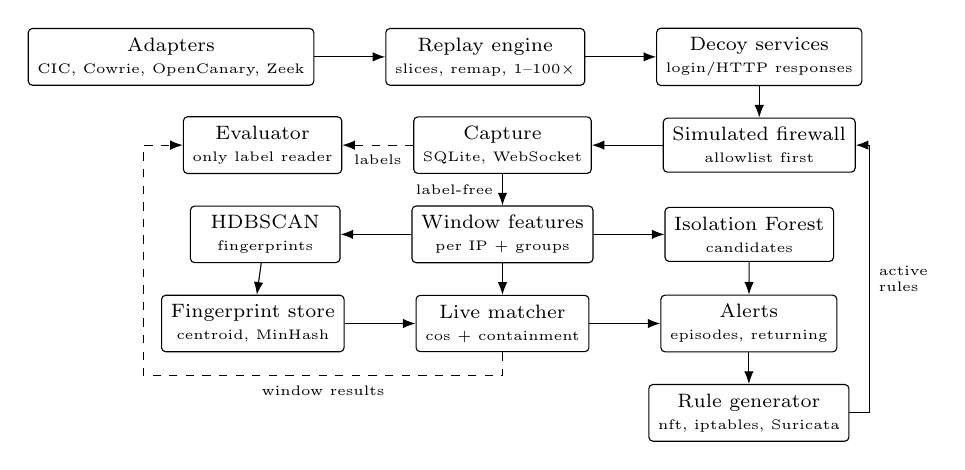
\begin{tikzpicture}[font=\scriptsize, node distance=4mm and 9mm,
  box/.style={draw, rounded corners=1.5pt, align=center, minimum width=19mm, minimum height=6mm, fill=white},
  lay/.style={font=\tiny\bfseries, text=black!60},
  arr/.style={-{Latex[length=1.6mm]}, thin}]
\node[box] (ad) {Adapters\\{\tiny CIC, Cowrie, OpenCanary, Zeek}};
\node[box, right=of ad] (re) {Replay engine\\{\tiny slices, remap, 1--100$\times$}};
\node[box, right=of re] (dc) {Decoy services\\{\tiny login/HTTP responses}};
\node[box, below=of dc] (fw) {Simulated firewall\\{\tiny allowlist first}};
\node[box, left=of fw] (cap) {Capture\\{\tiny SQLite, WebSocket}};
\node[box, left=of cap] (ev) {Evaluator\\{\tiny only label reader}};
\node[box, below=of cap] (fx) {Window features\\{\tiny per IP + groups}};
\node[box, right=of fx] (if) {Isolation Forest\\{\tiny candidates}};
\node[box, left=of fx] (hd) {HDBSCAN\\{\tiny fingerprints}};
\node[box, below=of fx] (mt) {Live matcher\\{\tiny cos + containment}};
\node[box, right=of mt] (al) {Alerts\\{\tiny episodes, returning}};
\node[box, left=of mt] (fp) {Fingerprint store\\{\tiny centroid, MinHash}};
\node[box, below=of al] (rg) {Rule generator\\{\tiny nft, iptables, Suricata}};
\draw[arr] (ad)--(re); \draw[arr] (re)--(dc); \draw[arr] (dc)--(fw); \draw[arr] (fw)--(cap);
\draw[arr] (cap)--node[left, font=\tiny, align=right]{label-free}(fx);
\draw[arr, dashed] (cap)--node[below, font=\tiny]{labels}(ev);
\draw[arr] (fx)--(mt); \draw[arr] (fx)--(if); \draw[arr] (fx)--(hd);
\draw[arr] (hd)--(fp); \draw[arr] (fp)--(mt); \draw[arr] (mt)--(al); \draw[arr] (if)--(al);
\draw[arr] (al)--(rg);
\draw[arr] (rg.east) -- ++(2.5mm,0) |- node[pos=0.25, right, font=\tiny, align=left]{active\\rules} (fw.east);
\draw[arr, dashed] (mt.south) -- ++(0,-3mm) -| node[pos=0.25, below, font=\tiny]{window results} ([xshift=-5mm]ev.west) -- (ev.west);
\end{tikzpicture}
\caption{Architecture. Adapters and replay stand in for the deception and collection layers (L1--L2), feature extraction for L3, HDBSCAN and the fingerprint store for L4, matching and alerts for L5, and rules with the simulated firewall for L6. Dashed edges carry ground truth and window results to the evaluator only.}
\label{fig:arch}
\end{figure*}

\section{Data Model and Input Adapters}\label{sec:data}
\subsection{Event schema and label isolation}
An event is $e=(t, \mathit{src}, \mathit{dst}, \mathit{svc}, \mathit{proto}, \mathbf{f}, \mathbf{h}, \mathbf{a}, \mathbf{c}, y, \kappa)$. It holds timestamps and endpoints; flow totals $\mathbf{f}$ (duration, forward and backward packets, bytes, SYN/ACK/FIN/RST/PSH counts); HTTP fields $\mathbf{h}$ (method, path, user agent, status); authentication fields $\mathbf{a}$ (username, password, attempt, outcome); and content $\mathbf{c}$ (command, payload snippet). The ground-truth label $y$ and campaign identifier $\kappa$ are kept verbatim from the source. Any field a source does not provide is \texttt{None}. The detection pipeline receives a separate type, \texttt{ObservedEvent}, which has no $y$ or $\kappa$ field, so a component cannot read a label even by mistake; a unit test checks this.

\subsection{Adapters}
\textit{CICFlowMeter CSV} (CIC-IDS2017\footnote{\url{https://www.unb.ca/cic/datasets/ids-2017.html}}, CIC-DDoS2019\footnote{\url{https://www.unb.ca/cic/datasets/ddos-2019.html}}). Each row, a bidirectional flow, becomes one flow event. Headers are matched after stripping whitespace, against both the 2017 and the newer CICFlowMeter spellings. \texttt{Infinity} and \texttt{NaN} become missing. CIC-IDS2017 writes afternoon times on a 12-hour clock without AM/PM, so hours 1--7 are shifted by 12~h. Minute-resolution timestamps are spread evenly across the minute in file order. The variant without source IP and timestamp columns is rejected with an explanatory error.
\textit{Cowrie}\footnote{\url{https://docs.cowrie.org/}}. Connect, login success and failure, command, download and session-close events are mapped, and source ports are carried from each session's connect event to its later events.
\textit{OpenCanary}\footnote{\url{https://github.com/thinkst/opencanary}}. Port-scan log types (5001--5005) become probe events whose flags are taken from the key set of the kernel log, and SSH, FTP, HTTP, MySQL and other login types become authentication attempts with an unresolved outcome. Boot and system messages are ignored.
\textit{Zeek conn.log}\footnote{\url{https://zeek.org/}}. TSV with a \texttt{\#fields} header or JSON lines are accepted. Flag counts are derived from the connection \texttt{history} string. IoT-23 \texttt{conn.log.labeled} files\footnote{\url{https://www.stratosphereips.org/datasets-iot23}}, whose last columns are joined by spaces, are split correctly, and their \texttt{detailed-label} becomes $y$.

\subsection{Label mapping and coverage}
One table maps normalised dataset labels to 19 behaviour keys (Table~\ref{tab:labels}). Behaviours that no supported labelled dataset provides are marked \emph{no data source} instead of being simulated. These are search-engine crawler, aggressive scraper, ICMP flood and stealthy port scan, plus credential stuffing and post-login shell activity, which appear in Cowrie and OpenCanary logs but carry no label; a replay can attach a label to such a slice explicitly.

\begin{table}[t]
\centering
\caption{Dataset-label to behaviour mapping (excerpt)}
\label{tab:labels}
\footnotesize
\begin{tabular}{@{}p{43mm}l@{}}
\toprule
Dataset labels & Behaviour \\
\midrule
DoS Hulk, DoS GoldenEye, DDoS (2017), WebDDoS & HTTP flood \\
DoS slowloris, DoS Slowhttptest & Slowloris \\
PortScan; PartOfAHorizontalPortScan (IoT-23) & Port scan (fast) \\
SSH-Patator / FTP-Patator & SSH / FTP brute force \\
Web Attack -- Brute Force & Web login brute force \\
Web Attack -- XSS, Sql Injection & Web vuln probing \\
Syn (2019) & SYN flood \\
DrDoS\_*, UDP, UDP-lag, TFTP, LDAP, \ldots & UDP flood / amplification \\
Bot; C\&C*, Okiru (IoT-23) & Botnet / C2 \\
Infiltration, Heartbleed & Infiltration \\
\midrule
\multicolumn{2}{@{}p{80mm}@{}}{\emph{No data source:} crawler, scraper, ICMP flood, stealthy scan, credential stuffing, post-login shell.}\\
\bottomrule
\end{tabular}
\end{table}

\section{Deterministic Replay Engine}\label{sec:replay}
A \emph{selection} names a source, optional label and time filters, an offset $o$ on the replay timeline, a compression factor $c$ (dataset seconds per replay second), a row cap, a sampling stride, an optional label override and an optional loop count. A dataset event at time $t_d$ in a slice starting at $t_0$ is scheduled at replay time $r=o+(t_d-t_0)/c$ and stamped $t=b+r$, where $b$ is the wall-clock time at which the replay starts, so replayed timestamps are shifted to the present. All selections are merged in a heap keyed by $r$. The engine advances in fixed steps of $\Delta=0.25$~s regardless of wall-clock speed (Algorithm~\ref{alg:replay}), so a plan always produces the same event sequence and the same results. A unit test checks that step sizes of 0.1, 1 and 5~s yield identical output. When the processing thread falls behind the requested speed, the replay clock slows down instead of skipping events.

\begin{algorithm}[t]
\caption{Deterministic replay step}\label{alg:replay}
\small
\begin{algorithmic}[1]
\Require heap $Q$ of $(r, k, e)$; clock $r_c$; base $b$; script $\Sigma$
\State $r_1 \gets r_c+\Delta$;\ $E\gets\emptyset$
\While{$Q\neq\emptyset$ \textbf{and} $\min(Q).r<r_1$}
  \State $(r,k,e)\gets \textsc{Pop}(Q)$;\ $e.t\gets b+r$;\ $E\gets E\cup\{e\}$
\EndWhile
\State fire every unfired step $s\in\Sigma$ with $s.r<r_1$ \Comment{narrate, mode, cluster}
\State $r_c\gets r_1$;\ \Return $E$
\end{algorithmic}
\end{algorithm}

\textit{Returning-attacker mode} (Algorithm~\ref{alg:returning}) takes the records of one attack class in time order and splits them at fraction $\phi$. Part A replays with its original addresses after a benign baseline. Part B replays after a gap longer than the episode gap, with every source address $a$ replaced by $\rho_s(a)$: a deterministic, injective-in-practice remapping derived from a keyed BLAKE2b hash with seed $s$, so all records from one original source keep one new address. Both parts share one compression factor, so their rates stay comparable. Slices too short to fill several windows can be looped back-to-back; benign background loops receive fresh addresses on each copy, so that a handful of hosts does not turn into periodic beacons. Every plan reports when this happened.

\begin{algorithm}[t]
\caption{Returning-attacker plan}\label{alg:returning}
\small
\begin{algorithmic}[1]
\Require records $R$ of class $\ell$ sorted by time; split $\phi$; target length $T_A$; gap $g$; baseline $T_0$; seed $s$
\State $n_A\gets\lfloor\phi|R|\rfloor$;\ $A\gets R_{1..n_A}$;\ $B\gets R_{n_A+1..|R|}$
\State $m_A\gets\lceil 60/|A|\rceil$, $m_B\gets\lceil 60/|B|\rceil$ \Comment{loop counts}
\State $c\gets \mathrm{span}(A, m_A)/T_A$ \Comment{shared compression}
\State $o_A\gets T_0$;\ $o_B\gets o_A+\mathrm{span}(A,m_A)/c+g$
\State add benign background spanning the plan, looped with fresh IPs if short
\State add $(A, o_A, c, m_A)$ with campaign $\kappa_A$
\State add $(B, o_B, c, m_B, \text{remap}=\rho_s)$ with campaign $\kappa_B$, parent $\kappa_A$
\State script: force clustering at the end of $A$
\end{algorithmic}
\end{algorithm}

\section{Flow-Aware Behavioural Features}\label{sec:features}
Every hop $H=5$~s, events in the trailing window $W=10$~s are grouped into \emph{entities}. A source IP becomes an entity when it has at least $n_{\min}=3$ events in the window or at least $4n_{\min}$ events in a 300~s history. Otherwise its events join a \emph{campaign-cluster group} keyed by traffic shape: protocol, service, well-known port and a request class (SYN-only, RST, established, authentication, HTTP page or sensitive path, command). Groups with at least three events form an entity. This is how spoofed SYN floods and distributed credential attacks, which produce one or two events per source, become visible. For each entity we compute the 49 features of Table~\ref{tab:features}. Count and rate features are transformed by $\tilde x=\log(1+x)$~\cite{savage2025}. Two examples:
\begin{align}
\mathrm{half\_open}&=|\mathcal T_{\mathrm{ho}}|\,/\,|\mathcal T|,\\
\mathrm{reply}&=\log\big(1+\operatorname{mean}_{e\in\mathcal F}\, b_e/\max(1,f_e)\big),
\end{align}
where $\mathcal T$ are the TCP events with flag information, $\mathcal T_{\mathrm{ho}}\subseteq\mathcal T$ those with SYN but no ACK and no reply packets, and $f_e,b_e$ are the forward and backward packets of the flows $\mathcal F$ that report both. Inter-arrival statistics use the window, or the long history when the window has fewer than three events. We use $\mathrm{CV}=\sigma/\mu$ and burstiness $B=(\sigma-\mu)/(\sigma+\mu)$.

\textit{Missing values.} A feature that a source cannot observe is NaN, not zero. Flag ratios are undefined for Cowrie logins, and HTTP ratios are undefined for CIC flows. After scaling, NaN becomes 0, the baseline, so it contributes nothing to similarity, and the categoriser skips it. Treating ``not observed'' as ``zero'' would make, for example, every Cowrie window look like a perfect non-SYN-flood.

\textit{Categorical traits.} Each entity also carries token sets in ten families: service and event type, top ports and a port-spread bucket, flag shapes, log$_2$ size buckets, paths, user agents, usernames, passwords, command verbs and command bigrams per session, and payload tokens.

\begin{table}[t]
\centering
\caption{Numeric feature families (49 features)}
\label{tab:features}
\footnotesize
\begin{tabular}{@{}lp{58mm}@{}}
\toprule
Family & Features \\
\midrule
Volume & events/s, packets/s, bytes/s, connections/s (log) \\
Protocol & TCP/UDP/ICMP ratio, SYN ratio, SYN:ACK, RST ratio, half-open ratio \\
Flow shape & duration, packets/flow, bytes/flow, reply ratio \\
Packets & size mean, size std, size entropy \\
Timing & IAT mean, IAT std, CV, burstiness \\
Breadth & unique dst ports, dst IPs, paths, users, passwords; src-port diversity \\
Auth & auth ratio, fail rate, fail ratio, success-after-fail, user diversity \\
HTTP & HTTP ratio, error ratio, UA diversity, path entropy, sensitive-path ratio \\
Content & command count, command ratio \\
Service & web, SSH/Telnet, FTP, DNS ratios \\
Sources & long-horizon ports, events, dst IPs; number of sources; rate per source \\
\bottomrule
\end{tabular}
\end{table}

\section{Fingerprinting}\label{sec:fingerprint}
\subsection{Scaling}
A StandardScaler fitted on the recent window buffer supplies the spread, floored at $0.2$ so that near-constant features cannot dominate. The centre is the mean of a benign baseline period (the first 30~s of a replay), so normal traffic sits near the origin:
\begin{equation}
z_j=\operatorname{clip}\!\Big(\frac{x_j-\mu^{\mathrm{base}}_j}{\max(\sigma^{\mathrm{buf}}_j,0.2)},\,-8,\,8\Big),\qquad z_j\gets0\text{ if }x_j=\mathrm{NaN}.
\end{equation}

\subsection{Clustering: HDBSCAN rather than DBSCAN}
Behaviour densities differ by orders of magnitude: a flood produces hundreds of near-identical windows, a scan a handful. DBSCAN's single $\varepsilon$ either merges sparse groups or splits dense ones. HDBSCAN (the scikit-learn implementation) keeps the most stable clusters across densities, needs no $k$, and labels leftovers as noise, which remain unassigned and may become anomaly candidates. Every 15~s, the clustering pass in Algorithm~\ref{alg:cluster} runs on unassigned windows only. Before clustering, it re-matches leftover windows against existing fingerprints, so that stragglers from an already-known behaviour do not seed a mixed cluster with a newer one. We found this failure mode during development.

\begin{algorithm}[t]
\caption{Clustering pass and fingerprint placement}\label{alg:cluster}
\small
\begin{algorithmic}[1]
\Require buffer $\mathcal B$; store $\mathcal S$; threshold $\theta$
\State re-categorise fingerprints whose centroid drifted
\State $U\gets\{w\in\mathcal B: w.\mathit{fp}=\varnothing\}$; refit spread on $\mathcal B$
\For{$w\in U$} \Comment{absorb leftovers}
  \State $(F,s)\gets\arg\max_{F\in\mathcal S_{\mathrm{active}}}\mathrm{sim}(w,F)$;\ \textbf{if} $s\ge\theta$ \textbf{then} $\textsc{Update}(F,\{w\})$
\EndFor
\State $L\gets\mathrm{HDBSCAN}(z(U'), m_{\mathrm{cs}}{=}5, m_{\mathrm{s}}{=}3)$ on the remaining $U'$
\For{each cluster $C$ with label $\ge0$}
  \State $(F,s)\gets\arg\max_{F\in\mathcal S}\mathrm{sim}(\bar C, F)$ \Comment{active, candidate, dismissed}
  \If{$s\ge\theta-0.05$}
    \If{$F$ dismissed} mark $C$ suppressed
    \Else\ $\textsc{Update}(F,C)$; promote $F$ if candidate and $|C|\ge m_{\mathrm{cs}}$ \EndIf
  \Else\ $F\gets\textsc{Create}(C)$: centroid, spread, tokens, MinHash, category, episode
  \EndIf
\EndFor
\end{algorithmic}
\end{algorithm}

\subsection{Fingerprint model}
A fingerprint stores a raw centroid and spread, token counts per family (at most 400), a 128-permutation MinHash signature, importance as $z$-scores against the baseline, source, ASN and country counters, a list of episodes, a version history and a hit timeline. MinHash uses $h_i(x)=\mathrm{SplitMix64}(\mathrm{hash}(x)\oplus s_i)$ with 128 random seeds. An earlier variant of the form $(a x+b)\bmod p$, with 31-bit coefficients on 32-bit hashes, barely wraps modulo $p$, so it is close to a monotone map. It estimated a true Jaccard of $1/3$ as 0.16, and the SplitMix64 version passes the same test. Live matches nudge the centroid with an exponential moving average ($\alpha=0.02$) and add tokens, so fingerprints keep learning.

\subsection{Explainable categoriser}
Each behaviour has one or more condition lists over centroid features (e.g.\ SYN flood: half-open ratio $\ge0.7$; packets/flow $\le3$; $\ge$20 flows/s; random source ports). The first condition, and any marked as required, must be observable and satisfied. Let $E$ be the observable conditions of a list with $n$ conditions and $M\subseteq E$ those satisfied. The confidence is
\begin{equation}
\gamma=\frac{|M|}{|E|}\Big(0.85+0.15\frac{|E|}{n}\Big),\quad |E|\ge n/2,
\end{equation}
rounded to four decimals. Without rounding, a 3-of-4 score falls just under the 0.75 cut-off in floating point, which we observed. The best list wins if $\gamma\ge0.75$. Otherwise the fingerprint is \emph{benign} when the mean $|z|$ of its centroid against the baseline is below 1, and \emph{unknown anomaly} when it is not. The matched and unmatched condition texts are kept as the explanation.

\subsection{Similarity}
For a live window $w$ and a fingerprint $F$ with scaled vectors $\mathbf z_w,\mathbf z_F$:
\begin{align}
\cos^{\!*}(w,F)&=\max\!\Big(0,\frac{[\mathbf z_w;\eta]\cdot[\mathbf z_F;\eta]}{\|[\mathbf z_w;\eta]\|\,\|[\mathbf z_F;\eta]\|}\Big),\ \eta=2,\label{eq:cos}\\
J^{\subset}(w,F)&=\frac{1}{|\Phi_w|}\sum_{\phi\in\Phi_w}\frac{|T_w^\phi\cap T_F^\phi|}{|T_w^\phi|},\label{eq:cont}\\
S(w,F)&=\frac{w_n\cos^{\!*}+w_c J^{\subset}}{w_n+w_c},\quad w_n=0.6,\ w_c=0.4.\label{eq:score}
\end{align}
The constant \emph{anchor} dimension $\eta$ in (\ref{eq:cos}) makes low-energy, baseline-like vectors point along the anchor instead of in arbitrary directions, while strong behaviours are compared by the direction of their deviation. A replay at a different rate along the same direction therefore keeps a high score. A 10~s window holds a small sample of a fingerprint's traits, so plain Jaccard would penalise it for being small. We therefore use containment (\ref{eq:cont}), averaged over the token families $\Phi_w$ present in the window, and keep the MinHash Jaccard estimate for fingerprint-to-fingerprint comparison. When a window has no tokens, $S=\cos^{\!*}$. Every match records its explanation: per-feature contributions $z_{w,j}z_{F,j}/(\|\cdot\|\|\cdot\|)$, the most divergent features, containment per family, and known versus new tokens.

\section{Detection, Episodes and Alerts}\label{sec:detect}
Algorithm~\ref{alg:match} processes each hop. A window whose best active fingerprint scores $S\ge\theta=0.85$ is a match. Otherwise an Isolation Forest (scikit-learn), trained on the baseline windows (150 trees, contamination 0.03), flags anomalies. An anomalous window joins a similar candidate fingerprint ($S\ge\theta-0.1$) or creates one, at most three per hop; candidates are promoted when a dense cluster confirms them, or by the user.

\textit{Episodes and returning behaviour.} An episode of $F$ is a maximal run of matches separated by less than a gap $g_e=25$~s. When a match opens a new episode $\epsilon_k$ with source set $I_k$,
\begin{equation}
\mathrm{returning}(\epsilon_k)\iff k>1\ \wedge\ I_k\cap\textstyle\bigcup_{j<k}I_j=\varnothing .\label{eq:ret}
\end{equation}
The behaviour is then known but its sources are not, which is the signature of an attacker who rotated infrastructure~\cite{savage2025,lim2026}.

\textit{Alerts} are keyed by (type, fingerprint, episode) and deduplicated within 120~s. The severity rank of an alert hit $n$ times is
\begin{equation}
\mathrm{sev}(n)=\min\!\big(\mathrm{sev}_0+[n\ge10]+[n\ge50],\ \textsc{critical}\big).
\end{equation}
Returning alerts start at least at \textsc{high}. Categories that resolve to benign never alert.

\begin{algorithm}[t]
\caption{Live matching, episodes and returning detection}\label{alg:match}
\small
\begin{algorithmic}[1]
\Require windows $\mathcal W$ at time $t$; active fingerprints $\mathcal S$; IF model
\For{$w\in\mathcal W$}
  \State $(F,s)\gets\arg\max_{F\in\mathcal S}S(w,F)$
  \If{$s\ge\theta$}
    \State $\epsilon\gets$ current episode of $F$
    \If{$\epsilon$ exists \textbf{and} $t-\epsilon.\mathit{end}\le g_e$} $\epsilon.I\gets\epsilon.I\cup w.I$
    \Else\ open $\epsilon'$ with $I=w.I$; $\epsilon'.\mathit{ret}\gets$ condition (\ref{eq:ret})
    \EndIf
    \State raise \textsc{returning} if $\epsilon.\mathit{ret}$ else \textsc{match}; \textsc{RuleFor}$(F,\epsilon)$
  \ElsIf{$\mathrm{IF}(z_w)<0$}
    \State join or create candidate; raise \textsc{anomaly}
  \EndIf
  \State append $w$ to the clustering buffer
\EndFor
\end{algorithmic}
\end{algorithm}

\section{Rule Generation and Simulated Enforcement}\label{sec:rules}
Each (fingerprint, episode) gets at most one rule, whose kind depends on the category (Table~\ref{tab:strategy}). The rule records its fingerprint, reason, creation time, expiry and history. It is rendered as nftables (sets with timeouts, meters), iptables (ipset, \texttt{hashlimit}, \texttt{connlimit}) and Suricata (\texttt{threshold}, \texttt{http.uri} and \texttt{http.user\_agent} content). New sources of the same episode extend the rule instead of creating another. The lifecycle is \emph{suggested}$\to$\emph{approved}$\to$\emph{active}$\to$\emph{expired}/\emph{rejected}. In suggest mode an analyst approves rules; in auto mode they activate immediately, except unknown-anomaly rules, which are never auto-applied.

\textit{Allowlist invariant.} Allowlisted CIDRs are removed from every rule target, including later user edits. The simulated firewall checks the allowlist before any rule, including rate limits, so an allowlisted source is never dropped. Rate rules use token buckets: with rate $\lambda$ and burst $2\lambda$, an event at time $t$ passes if $\min(2\lambda, b+\lambda(t-t'))\ge1$, where $b$ is the bucket level at the previous event $t'$. Dropped events are counted per rule and kept out of detection, which lets the dashboard show traffic before and after enforcement. No rule is ever executed on a host.

\begin{table}[t]
\centering
\caption{Rule strategy per behaviour category}
\label{tab:strategy}
\footnotesize
\resizebox{\columnwidth}{!}{%
\begin{tabular}{@{}ll@{}}
\toprule
Category & Rule kind \\
\midrule
SYN / UDP / ICMP flood & SYN rate limit / UDP port limit / ICMP limit \\
HTTP flood, credential stuffing & IP-set block with timeout \\
Slowloris & connection limit + source block \\
Scans, SSH/FTP/web brute force, C2 & IP block (IP set above 20 sources) \\
Web probing, post-login shell, malware & Suricata content + IP block \\
Unknown anomaly & IP block, suggest-only \\
\bottomrule
\end{tabular}}
\end{table}

\section{Implementation and Web Application}\label{sec:impl}
\subsection{Software stack and deployment}
The backend is a Python~3.11 FastAPI service. Events, fingerprints, alerts and rules are persisted in SQLite (write-ahead logging, buffered writes) through SQLModel, and NumPy, pandas and scikit-learn provide the numerical components. The detection pipeline runs in one background thread under a re-entrant lock, and a WebSocket pushes a batched state update to every client four times per second. The frontend is a React~18 single-page application built with Vite and Tailwind CSS, with Recharts for charts and a virtualised event table. One \texttt{docker compose up} starts both services: the backend on port 8000 with the data folder mounted read-only, and the frontend served by nginx on port 5173, which proxies \texttt{/api} and \texttt{/ws} to the backend. A non-Docker path runs the same two processes from a Python virtual environment and the Vite development server. The backend has 61 unit and integration tests (adapters, label table, replay determinism, features, fingerprinting, returning detection, rules and API), and the frontend has unit tests and a browser smoke test.

\subsection{Safety properties}
The application never opens a raw socket or sends a request to any host: replayed records are generated in-process from files, and the dashboard states this on every page. Rules are rendered as text for nftables, iptables and Suricata and can be exported, but no command is executed on the host; the \emph{enforcement} switch only changes the simulated firewall that filters the replayed stream. GeoIP and ASN data come from a bundled offline mock.

\subsection{Views}
The application has seven views, which also served as our measurement instrument (Section~\ref{sec:eval}).
\begin{itemize}
\item \emph{Replay control} (Fig.~\ref{fig:ui-replay}) lists the indexed data sources with their labels and mapped behaviours, and starts the scripted demonstration, a returning-attacker replay (source, class, split, part-A length, gap, speed) or a custom mix of slices. Pause, resume, stop and 1/10/100$\times$ speed apply at any time; the status bar shows replay time, effective speed, rule mode and the latest narration step.
\item \emph{Live overview} (Fig.~\ref{fig:ui-overview}) shows key indicators, a stacked chart of events per second coloured by the behaviour family that their source was last detected as, rule activations, traffic dropped by the simulated firewall, source countries from the mock GeoIP, and a live event table.
\item \emph{Fingerprint explorer} (Fig.~\ref{fig:ui-fp}) projects windows and fingerprint centroids with PCA or t-SNE, lists fingerprints by status and opens a detail panel with a radar profile, distinguishing features, traits, episodes and history; fingerprints can be renamed, promoted, dismissed, merged or split.
\item \emph{Alerts} (Fig.~\ref{fig:ui-alerts}) is a filterable feed in which every alert expands into its explanation: the score breakdown of~(\ref{eq:score}), the strongest shared and most divergent features with their $z$-scores, containment per token family, and known versus new traits.
\item \emph{Firewall rules} (Fig.~\ref{fig:ui-rules}) holds the rule lifecycle, the suggest/auto switch, per-format text with an editor, parameters, history, export and the allowlist.
\item \emph{Evaluation} (Fig.~\ref{fig:ui-cm}) shows attack-versus-benign scores, a confusion matrix online and after clustering, per-behaviour scores, ground-truth campaigns with times to detect and to rule, and returning-attacker recognition.
\item \emph{Settings} exposes every parameter of Sections~\ref{sec:features}--\ref{sec:rules}.
\end{itemize}

\begin{figure*}[t]
\centering
\shot[trim=446 648 0 0, clip]{figures/web_replay_running.png}
\caption{Replay control during the scripted demonstration at 10$\times$ (application screenshot). The status bar narrates the current step; here the rule for the new SSH brute-force fingerprint has just been suggested. The returning-attacker panel configures source, class, split, part-A length, gap and speed.}
\label{fig:ui-replay}
\end{figure*}

\begin{figure*}[t]
\centering
\shot[trim=446 446 0 0, clip]{figures/web_rules.png}
\caption{Firewall rules after the demonstration (application screenshot): R-0001, suggested while the application was in suggest mode, with its nftables rendering and parameters (source, port 22, 900~s timeout, threshold 5 per 60~s); the episode rule R-0002 for the returning source is active. Allowlisted ranges are listed below the rules.}
\label{fig:ui-rules}
\end{figure*}

\begin{figure*}[t]
\centering
\shot[trim=446 490 0 0, clip]{figures/web_overview.png}
\caption{Live overview at the end of the scripted demonstration (application screenshot). Events per second are stacked by the detected family of their source: grey benign, red unknown-anomaly candidates during the baseline, green SSH brute force once the fingerprint exists. The dashed green line marks activation of rule R-0002 for the returning source, and the black dashed curve the events dropped by the simulated firewall from then on (58 of 2,123 in total).}
\label{fig:ui-overview}
\end{figure*}

\begin{figure*}[t]
\centering
\shot[trim=446 619 0 0, clip]{figures/web_alerts.png}
\caption{Alert feed with the returning-behaviour alert expanded (application screenshot). The explanation reports the combined score $0.938=0.6\times0.897+0.4\times1.000$, the strongest shared features (packets per flow, burstiness, SSH ratio) with live and fingerprint $z$-scores, the most divergent features, and trait containment per family. Below it are the earlier match, new-fingerprint and anomaly alerts with their hit counts.}
\label{fig:ui-alerts}
\end{figure*}

\begin{figure}[t]
\centering
\shot[trim=497 576 50 245, clip]{figures/web_mixed_fingerprints.png}
\caption{Fingerprint explorer after the mixed replay (PCA of window features; application screenshot). Diamonds are fingerprint centroids, dots are windows coloured by the family of their fingerprint; benign fingerprints cluster on the left, floods, scans, brute force, C2 and web probing separate to the right.}
\label{fig:ui-fp}
\end{figure}

\section{Evaluation Methodology}\label{sec:eval}
\textit{Research questions.} RQ1: Does a fingerprint learned from one part of an attack recognise the same behaviour when it returns from new addresses, and how quickly? RQ2: How accurately are windows classified into behaviours, online and after clustering, and where do errors fall? RQ3: What does automatic enforcement change? RQ4: Which design choices matter (ablations)? RQ5: What does the pipeline cost?

\textit{Data.} The full datasets were not available when we ran these experiments, so all results use the bundled sample files: two CICFlowMeter CSVs with real CIC-IDS2017 and CIC-DDoS2019 headers (50 and 40 rows), a Cowrie log (28 events), an OpenCanary log (27), an IoT-23-style labelled Zeek TSV (30) and a Zeek JSON log (20). They are \emph{synthesised} in each tool's real format, with labels drawn from the datasets' vocabularies, and the replay engine loops them. Such ground truth has known weaknesses~\cite{oliveira2026,aparna2026}: these labels are independent of the detector, but the data is small, synthetic and repetitive. Looping produces artefacts that real data would not have, such as repeated source ports and perfectly periodic timing.

\textit{Two measurement paths.} \emph{(i) Web application.} Results W1--W2 were measured on the deployed Docker stack through its own interface. A script (\texttt{paper/tools/capture\_site.py}) resets the application, starts a scenario through the same REST endpoints that the Replay view calls, waits for the replay to finish, saves the JSON behind the Evaluation, Overview, Alerts and Rules views, and takes the screenshots shown in this paper with a headless browser. W1 is the scripted demonstration at 10$\times$. W2 is an eight-slice mix of all six files at 100$\times$ with the rule mode left on \emph{auto-apply}, as the demonstration leaves it. Running the capture twice gave identical numbers. \emph{(ii) Headless harness.} Experiments E1--E6 call the same pipeline directly, without persistence or the network layer, in the default \emph{suggest} mode, which allows sweeps and ablations (\texttt{python -m experiments.paper\_experiments}). Both paths use the same evaluator.

\textit{Label provenance.} Window ground truth is the majority mapped label of the events a window contains. Cowrie and OpenCanary windows are unlabelled and excluded unless a replay overrides their label (W2 labels the Cowrie slice as SSH brute force and leaves OpenCanary unlabelled).

\textit{Metrics.} Let $C\in\mathbb N^{K\times K'}$ be the confusion matrix whose entry $C_{ij}$ counts windows with true behaviour $i$ and detected category $j$; the detected categories add \emph{unknown anomaly} and \emph{unclassified} (no fingerprint matched) to the behaviours. For behaviour $i$,
\begin{equation}
P_i=\frac{C_{ii}}{\sum_k C_{ki}},\quad R_i=\frac{C_{ii}}{\sum_j C_{ij}},\quad F_i=\frac{2P_iR_i}{P_i+R_i},
\end{equation}
macro F1 is the mean of $F_i$ over true behaviours, and accuracy is $\sum_i C_{ii}/\sum_{ij}C_{ij}$. We report $C$ \emph{online} (the category of the window's best fingerprint at detection time) and \emph{after clustering}, which credits windows that HDBSCAN later assigned to a fingerprint, using that fingerprint's current category. For attack-versus-benign detection a window is predicted \emph{attack} when it matched a non-benign fingerprint or was flagged anomalous, which gives TP, FP, FN, TN, precision, recall and F1. We also report the time to detect (first event of a campaign to its first flagged window) and the time to rule (to its first rule); returning-attacker recognition, meaning that a part-B window matched a fingerprint that part-A windows built or matched; whether a returning alert was raised; the similarity and the alert delay; and the share of events dropped. Finally we report throughput and per-stage latency.

\textit{Setup.} An Intel Core i5-1235U laptop with 15.7~GB RAM, Windows~11, Docker Desktop, Python 3.11.14, scikit-learn 1.5.2 and NumPy 2.1.3; screenshots were taken at 1440$\times$900 CSS pixels with device scale factor 2 in the light theme. Default settings throughout ($W=10$~s, $H=5$~s, $\theta=0.85$, $w_n{:}w_c=0.6{:}0.4$, HDBSCAN $m_{\mathrm{cs}}=5$, $m_{\mathrm{s}}=3$, clustering every 15~s). Every run is deterministic, so variation comes only from the split fraction and the remap seed.

\section{Results}\label{sec:results}
\subsection{W1: Scripted demonstration in the web application}
The demonstration replays a benign CIC-IDS2017 background from 600 rotating addresses, part A of the SSH-Patator class from its original address, a switch to auto-apply, and part B from a remapped address (Figs.~\ref{fig:ui-replay}--\ref{fig:ui-alerts}). Of 2,123 events, 977 labelled windows were evaluated. The application learned 10 fingerprints, nine of them benign plus \emph{SSH brute force \#1} (FP-0010). The alert feed contains five alerts: two low-severity unknown-anomaly candidates raised on benign windows during the baseline, the new-fingerprint alert, a match alert (score 0.996) and the returning-behaviour alert (score 0.938, numeric cosine 0.897, containment 1.000). Part B was recognised in its first hop: its time to detect and to rule were both 5.0~s, against 35.0~s and 30.0~s for part A, which had to wait for clustering. The episode rule R-0002 was auto-applied and dropped 58 of the 63 part-B events (92\%); R-0001, suggested before the switch, stayed suggested. Table~\ref{tab:web} and Fig.~\ref{fig:cm-demo} summarise the scores. Precision is 0.636 because the four baseline anomaly windows are false positives; after clustering, 964 of 964 benign and 12 of 13 SSH windows are attributed correctly.

\subsection{W2: Mixed replay under automatic enforcement}
Eight slices from all six files ran overlapping for 236~s of replay time: 7,528 events, of which the simulated firewall dropped 243 (143 SSH brute force including the Cowrie slice, 48 port scan, 34 C2, 18 OpenCanary probes). The application formed 18 fingerprints: nine benign and nine non-benign covering C2, SSH brute force (two, from CIC flows and from Cowrie logins), UDP flood, SYN flood (two), fast port scan, web vulnerability probing (from the unlabelled OpenCanary log) and one unknown anomaly. It raised 17 alerts and generated nine rules, eight active and one unknown-anomaly rule left suggested, as the auto mode requires.

Of 805 labelled windows, attack-versus-benign detection gave $\mathrm{TP}=39$, $\mathrm{FP}=0$, $\mathrm{FN}=10$, $\mathrm{TN}=756$: precision 1.000, recall 0.796, F1 0.886 (Table~\ref{tab:web}). Fig.~\ref{fig:cm-mixed} shows where the online errors fall. No attack window was ever assigned to a wrong attack class or to benign, and no benign window to an attack. All online errors lie in two columns. \emph{Unknown anomaly} holds 28 attack windows that the Isolation Forest flagged before a fingerprint for their behaviour existed: they count as detected attacks but not as correctly categorised. \emph{Unclassified} holds 147 benign windows and 10 attack windows (9 SSH, 1 C2) seen before the first clustering pass. Online macro F1 is therefore 0.458 at accuracy 0.770. After clustering the matrix is almost diagonal: two windows remain unclassified (one benign, one SSH), giving macro F1 0.995 and accuracy 0.998. Fig.~\ref{fig:ui-cm} shows the same matrices as the Evaluation view renders them.

\begin{table}[t]
\centering
\caption{W1--W2: Scores measured in the web application}
\label{tab:web}
\footnotesize
\setlength{\tabcolsep}{3pt}
\begin{tabular}{@{}lcc@{}}
\toprule
Measure & W1 demo (10$\times$) & W2 mixed (100$\times$, auto) \\
\midrule
Events / dropped & 2,123 / 58 & 7,528 / 243 \\
Labelled windows & 977 & 805 \\
Fingerprints (non-benign) & 10 (1) & 18 (9) \\
Alerts / active rules & 5 / 1 & 17 / 8 \\
TP / FP / FN / TN & 7 / 4 / 6 / 960 & 39 / 0 / 10 / 756 \\
Attack precision / recall & 0.636 / 0.538 & 1.000 / 0.796 \\
Attack F1 & 0.583 & 0.886 \\
Macro F1 online / final & 0.785 / 0.980 & 0.458 / 0.995 \\
Accuracy online / final & 0.768 / 0.999 & 0.770 / 0.998 \\
Mean time to detect / to rule & 20.0 / 17.5 s & 10.0 / 30.0 s \\
Returning recognised / alerted & 1 of 1 / 1 of 1 & -- \\
\bottomrule
\end{tabular}
\end{table}

\begin{figure*}[t]
\centering
\begin{minipage}[b]{0.39\textwidth}\centering
\resizebox{\linewidth}{!}{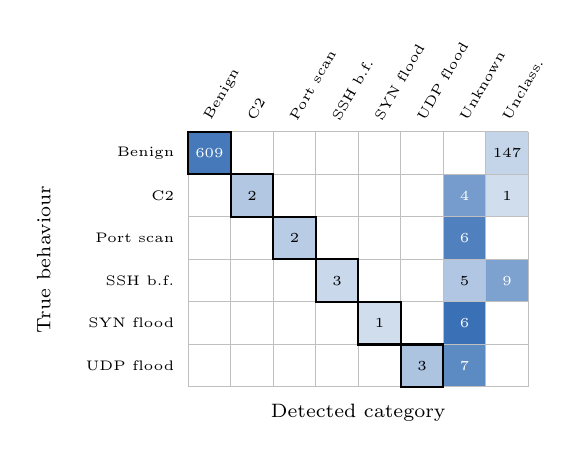
\begin{tikzpicture}[x=5.4mm,y=5.4mm,font=\tiny]
\node[anchor=east] at (-0.1,5.5) {Benign};
\fill[cmblue!82!white] (0,5) rectangle ++(1,1);
\node[text=white] at (0.5,5.5) {609};
\fill[white] (1,5) rectangle ++(1,1);
\fill[white] (2,5) rectangle ++(1,1);
\fill[white] (3,5) rectangle ++(1,1);
\fill[white] (4,5) rectangle ++(1,1);
\fill[white] (5,5) rectangle ++(1,1);
\fill[white] (6,5) rectangle ++(1,1);
\fill[cmblue!26!white] (7,5) rectangle ++(1,1);
\node[text=black] at (7.5,5.5) {147};
\node[anchor=east] at (-0.1,4.5) {C2};
\fill[white] (0,4) rectangle ++(1,1);
\fill[cmblue!34!white] (1,4) rectangle ++(1,1);
\node[text=black] at (1.5,4.5) {2};
\fill[white] (2,4) rectangle ++(1,1);
\fill[white] (3,4) rectangle ++(1,1);
\fill[white] (4,4) rectangle ++(1,1);
\fill[white] (5,4) rectangle ++(1,1);
\fill[cmblue!61!white] (6,4) rectangle ++(1,1);
\node[text=white] at (6.5,4.5) {4};
\fill[cmblue!21!white] (7,4) rectangle ++(1,1);
\node[text=black] at (7.5,4.5) {1};
\node[anchor=east] at (-0.1,3.5) {Port scan};
\fill[white] (0,3) rectangle ++(1,1);
\fill[white] (1,3) rectangle ++(1,1);
\fill[cmblue!31!white] (2,3) rectangle ++(1,1);
\node[text=black] at (2.5,3.5) {2};
\fill[white] (3,3) rectangle ++(1,1);
\fill[white] (4,3) rectangle ++(1,1);
\fill[white] (5,3) rectangle ++(1,1);
\fill[cmblue!77!white] (6,3) rectangle ++(1,1);
\node[text=white] at (6.5,3.5) {6};
\fill[white] (7,3) rectangle ++(1,1);
\node[anchor=east] at (-0.1,2.5) {SSH b.f.};
\fill[white] (0,2) rectangle ++(1,1);
\fill[white] (1,2) rectangle ++(1,1);
\fill[white] (2,2) rectangle ++(1,1);
\fill[cmblue!24!white] (3,2) rectangle ++(1,1);
\node[text=black] at (3.5,2.5) {3};
\fill[white] (4,2) rectangle ++(1,1);
\fill[white] (5,2) rectangle ++(1,1);
\fill[cmblue!35!white] (6,2) rectangle ++(1,1);
\node[text=black] at (6.5,2.5) {5};
\fill[cmblue!57!white] (7,2) rectangle ++(1,1);
\node[text=white] at (7.5,2.5) {9};
\node[anchor=east] at (-0.1,1.5) {SYN flood};
\fill[white] (0,1) rectangle ++(1,1);
\fill[white] (1,1) rectangle ++(1,1);
\fill[white] (2,1) rectangle ++(1,1);
\fill[white] (3,1) rectangle ++(1,1);
\fill[cmblue!21!white] (4,1) rectangle ++(1,1);
\node[text=black] at (4.5,1.5) {1};
\fill[white] (5,1) rectangle ++(1,1);
\fill[cmblue!87!white] (6,1) rectangle ++(1,1);
\node[text=white] at (6.5,1.5) {6};
\fill[white] (7,1) rectangle ++(1,1);
\node[anchor=east] at (-0.1,0.5) {UDP flood};
\fill[white] (0,0) rectangle ++(1,1);
\fill[white] (1,0) rectangle ++(1,1);
\fill[white] (2,0) rectangle ++(1,1);
\fill[white] (3,0) rectangle ++(1,1);
\fill[white] (4,0) rectangle ++(1,1);
\fill[cmblue!36!white] (5,0) rectangle ++(1,1);
\node[text=black] at (5.5,0.5) {3};
\fill[cmblue!72!white] (6,0) rectangle ++(1,1);
\node[text=white] at (6.5,0.5) {7};
\fill[white] (7,0) rectangle ++(1,1);
\draw[black!25, step=1] (0,0) grid (8,6);
\draw[black, thick] (0,5) rectangle ++(1,1);
\draw[black, thick] (1,4) rectangle ++(1,1);
\draw[black, thick] (2,3) rectangle ++(1,1);
\draw[black, thick] (3,2) rectangle ++(1,1);
\draw[black, thick] (4,1) rectangle ++(1,1);
\draw[black, thick] (5,0) rectangle ++(1,1);
\node[anchor=west, rotate=60] at (0.35,6.1) {Benign};
\node[anchor=west, rotate=60] at (1.35,6.1) {C2};
\node[anchor=west, rotate=60] at (2.35,6.1) {Port scan};
\node[anchor=west, rotate=60] at (3.35,6.1) {SSH b.f.};
\node[anchor=west, rotate=60] at (4.35,6.1) {SYN flood};
\node[anchor=west, rotate=60] at (5.35,6.1) {UDP flood};
\node[anchor=west, rotate=60] at (6.35,6.1) {Unknown};
\node[anchor=west, rotate=60] at (7.35,6.1) {Unclass.};
\node[rotate=90, font=\scriptsize] at (-3.4,3) {True behaviour};
\node[font=\scriptsize] at (4,-0.6) {Detected category};
\end{tikzpicture}
}\\[1mm]
{\footnotesize (a) Online, at detection time}
\end{minipage}\hfill
\begin{minipage}[b]{0.34\textwidth}\centering
\resizebox{\linewidth}{!}{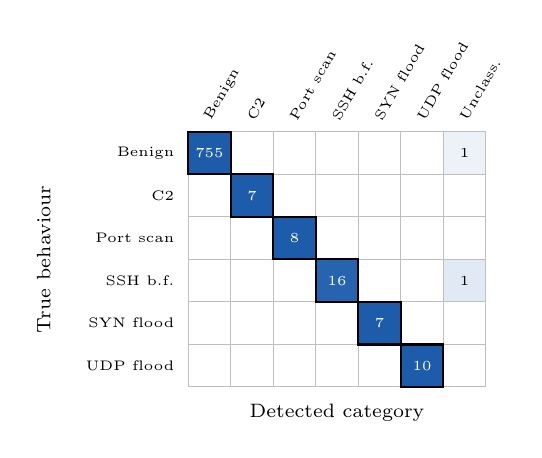
\begin{tikzpicture}[x=5.4mm,y=5.4mm,font=\tiny]
\node[anchor=east] at (-0.1,5.5) {Benign};
\fill[cmblue!100!white] (0,5) rectangle ++(1,1);
\node[text=white] at (0.5,5.5) {755};
\fill[white] (1,5) rectangle ++(1,1);
\fill[white] (2,5) rectangle ++(1,1);
\fill[white] (3,5) rectangle ++(1,1);
\fill[white] (4,5) rectangle ++(1,1);
\fill[white] (5,5) rectangle ++(1,1);
\fill[cmblue!8!white] (6,5) rectangle ++(1,1);
\node[text=black] at (6.5,5.5) {1};
\node[anchor=east] at (-0.1,4.5) {C2};
\fill[white] (0,4) rectangle ++(1,1);
\fill[cmblue!100!white] (1,4) rectangle ++(1,1);
\node[text=white] at (1.5,4.5) {7};
\fill[white] (2,4) rectangle ++(1,1);
\fill[white] (3,4) rectangle ++(1,1);
\fill[white] (4,4) rectangle ++(1,1);
\fill[white] (5,4) rectangle ++(1,1);
\fill[white] (6,4) rectangle ++(1,1);
\node[anchor=east] at (-0.1,3.5) {Port scan};
\fill[white] (0,3) rectangle ++(1,1);
\fill[white] (1,3) rectangle ++(1,1);
\fill[cmblue!100!white] (2,3) rectangle ++(1,1);
\node[text=white] at (2.5,3.5) {8};
\fill[white] (3,3) rectangle ++(1,1);
\fill[white] (4,3) rectangle ++(1,1);
\fill[white] (5,3) rectangle ++(1,1);
\fill[white] (6,3) rectangle ++(1,1);
\node[anchor=east] at (-0.1,2.5) {SSH b.f.};
\fill[white] (0,2) rectangle ++(1,1);
\fill[white] (1,2) rectangle ++(1,1);
\fill[white] (2,2) rectangle ++(1,1);
\fill[cmblue!95!white] (3,2) rectangle ++(1,1);
\node[text=white] at (3.5,2.5) {16};
\fill[white] (4,2) rectangle ++(1,1);
\fill[white] (5,2) rectangle ++(1,1);
\fill[cmblue!13!white] (6,2) rectangle ++(1,1);
\node[text=black] at (6.5,2.5) {1};
\node[anchor=east] at (-0.1,1.5) {SYN flood};
\fill[white] (0,1) rectangle ++(1,1);
\fill[white] (1,1) rectangle ++(1,1);
\fill[white] (2,1) rectangle ++(1,1);
\fill[white] (3,1) rectangle ++(1,1);
\fill[cmblue!100!white] (4,1) rectangle ++(1,1);
\node[text=white] at (4.5,1.5) {7};
\fill[white] (5,1) rectangle ++(1,1);
\fill[white] (6,1) rectangle ++(1,1);
\node[anchor=east] at (-0.1,0.5) {UDP flood};
\fill[white] (0,0) rectangle ++(1,1);
\fill[white] (1,0) rectangle ++(1,1);
\fill[white] (2,0) rectangle ++(1,1);
\fill[white] (3,0) rectangle ++(1,1);
\fill[white] (4,0) rectangle ++(1,1);
\fill[cmblue!100!white] (5,0) rectangle ++(1,1);
\node[text=white] at (5.5,0.5) {10};
\fill[white] (6,0) rectangle ++(1,1);
\draw[black!25, step=1] (0,0) grid (7,6);
\draw[black, thick] (0,5) rectangle ++(1,1);
\draw[black, thick] (1,4) rectangle ++(1,1);
\draw[black, thick] (2,3) rectangle ++(1,1);
\draw[black, thick] (3,2) rectangle ++(1,1);
\draw[black, thick] (4,1) rectangle ++(1,1);
\draw[black, thick] (5,0) rectangle ++(1,1);
\node[anchor=west, rotate=60] at (0.35,6.1) {Benign};
\node[anchor=west, rotate=60] at (1.35,6.1) {C2};
\node[anchor=west, rotate=60] at (2.35,6.1) {Port scan};
\node[anchor=west, rotate=60] at (3.35,6.1) {SSH b.f.};
\node[anchor=west, rotate=60] at (4.35,6.1) {SYN flood};
\node[anchor=west, rotate=60] at (5.35,6.1) {UDP flood};
\node[anchor=west, rotate=60] at (6.35,6.1) {Unclass.};
\node[rotate=90, font=\scriptsize] at (-3.4,3) {True behaviour};
\node[font=\scriptsize] at (3.5,-0.6) {Detected category};
\end{tikzpicture}
}\\[1mm]
{\footnotesize (b) After clustering}
\end{minipage}\hfill
\begin{minipage}[b]{0.24\textwidth}\centering
\resizebox{\linewidth}{!}{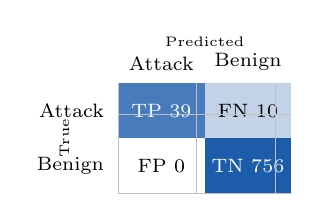
\begin{tikzpicture}[x=11mm,y=7mm,font=\scriptsize]
\fill[cmblue!81!white] (0,1) rectangle ++(1,1);
\node[text=white, align=center] at (0.5,1.5) {TP~39};
\fill[cmblue!27!white] (1,1) rectangle ++(1,1);
\node[text=black, align=center] at (1.5,1.5) {FN~10};
\node[anchor=east] at (-0.05,1.5) {Attack};
\node[anchor=south] at (0.5,2.05) {Attack};
\fill[white] (0,0) rectangle ++(1,1);
\node[text=black, align=center] at (0.5,0.5) {FP~0};
\fill[cmblue!100!white] (1,0) rectangle ++(1,1);
\node[text=white, align=center] at (1.5,0.5) {TN~756};
\node[anchor=east] at (-0.05,0.5) {Benign};
\node[anchor=south] at (1.5,2.05) {Benign};
\draw[black!25] (0,0) grid (2,2);
\node[font=\tiny] at (1,2.75) {Predicted};
\node[rotate=90, font=\tiny] at (-0.62,1) {True};
\end{tikzpicture}
}\\[1mm]
{\footnotesize (c) Attack vs.\ benign}
\end{minipage}
\caption{W2 confusion matrices measured in the web application (805 labelled windows of the mixed replay under auto-apply). Cells show window counts; shading is row-normalised; outlined cells are correct. Online errors fall only in the \emph{Unknown} and \emph{Unclass.} columns, i.e.\ before a fingerprint for the behaviour existed; no attack class is confused with another or with benign.}
\label{fig:cm-mixed}
\end{figure*}

\begin{figure}[t]
\centering
\begin{minipage}[b]{0.50\columnwidth}\centering
\resizebox{\linewidth}{!}{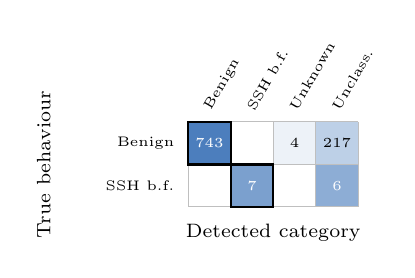
\begin{tikzpicture}[x=5.4mm,y=5.4mm,font=\tiny]
\node[anchor=east] at (-0.1,1.5) {Benign};
\fill[cmblue!79!white] (0,1) rectangle ++(1,1);
\node[text=white] at (0.5,1.5) {743};
\fill[white] (1,1) rectangle ++(1,1);
\fill[cmblue!8!white] (2,1) rectangle ++(1,1);
\node[text=black] at (2.5,1.5) {4};
\fill[cmblue!29!white] (3,1) rectangle ++(1,1);
\node[text=black] at (3.5,1.5) {217};
\node[anchor=east] at (-0.1,0.5) {SSH b.f.};
\fill[white] (0,0) rectangle ++(1,1);
\fill[cmblue!58!white] (1,0) rectangle ++(1,1);
\node[text=white] at (1.5,0.5) {7};
\fill[white] (2,0) rectangle ++(1,1);
\fill[cmblue!50!white] (3,0) rectangle ++(1,1);
\node[text=white] at (3.5,0.5) {6};
\draw[black!25, step=1] (0,0) grid (4,2);
\draw[black, thick] (0,1) rectangle ++(1,1);
\draw[black, thick] (1,0) rectangle ++(1,1);
\node[anchor=west, rotate=60] at (0.35,2.1) {Benign};
\node[anchor=west, rotate=60] at (1.35,2.1) {SSH b.f.};
\node[anchor=west, rotate=60] at (2.35,2.1) {Unknown};
\node[anchor=west, rotate=60] at (3.35,2.1) {Unclass.};
\node[rotate=90, font=\scriptsize] at (-3.4,1) {True behaviour};
\node[font=\scriptsize] at (2,-0.6) {Detected category};
\end{tikzpicture}
}\\[0.5mm]
{\footnotesize (a) Online}
\end{minipage}\hfill
\begin{minipage}[b]{0.46\columnwidth}\centering
\resizebox{\linewidth}{!}{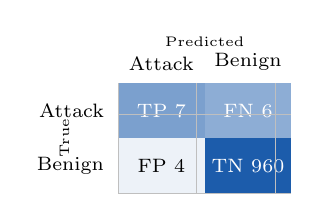
\begin{tikzpicture}[x=11mm,y=7mm,font=\scriptsize]
\fill[cmblue!58!white] (0,1) rectangle ++(1,1);
\node[text=white, align=center] at (0.5,1.5) {TP~7};
\fill[cmblue!50!white] (1,1) rectangle ++(1,1);
\node[text=white, align=center] at (1.5,1.5) {FN~6};
\node[anchor=east] at (-0.05,1.5) {Attack};
\node[anchor=south] at (0.5,2.05) {Attack};
\fill[cmblue!8!white] (0,0) rectangle ++(1,1);
\node[text=black, align=center] at (0.5,0.5) {FP~4};
\fill[cmblue!100!white] (1,0) rectangle ++(1,1);
\node[text=white, align=center] at (1.5,0.5) {TN~960};
\node[anchor=east] at (-0.05,0.5) {Benign};
\node[anchor=south] at (1.5,2.05) {Benign};
\draw[black!25] (0,0) grid (2,2);
\node[font=\tiny] at (1,2.75) {Predicted};
\node[rotate=90, font=\tiny] at (-0.62,1) {True};
\end{tikzpicture}
}\\[0.5mm]
{\footnotesize (b) Attack vs.\ benign}
\end{minipage}
\caption{W1 confusion matrices (977 windows of the scripted demonstration). After clustering (not shown) all 964 benign and 12 of 13 SSH windows are correct.}
\label{fig:cm-demo}
\end{figure}

\begin{figure*}[t]
\centering
\begin{minipage}[t]{0.495\textwidth}\centering
\shot{figures/web_mixed_cm_online.png}\\[0.5mm]{\footnotesize (a) Online}
\end{minipage}\hfill
\begin{minipage}[t]{0.495\textwidth}\centering
\shot{figures/web_mixed_cm_final.png}\\[0.5mm]{\footnotesize (b) After clustering}
\end{minipage}
\caption{The W2 confusion matrices as rendered by the application's Evaluation view (screenshots).}
\label{fig:ui-cm}
\end{figure*}

\textit{Per-campaign timing.} Table~\ref{tab:campaigns} lists the ground-truth campaigns of W2. Every labelled attack campaign was detected within 5--25~s of its first event and received a rule within 20--40~s. Enforcement dropped 27--67\% of the events of the brute-force, scan and C2 campaigns. The SYN and UDP flood slices are short (about 28~s and 42~s of replay) and their rate-limit rules became active 35~s and 40~s after their first events, so almost no flood traffic was left to drop. The unlabelled OpenCanary slice received a web-probing rule after 15~s.

\begin{table}[t]
\centering
\caption{W2: Ground-truth campaigns in the web application}
\label{tab:campaigns}
\footnotesize
\setlength{\tabcolsep}{2.5pt}
\resizebox{\columnwidth}{!}{%
\begin{tabular}{@{}llrrrr@{}}
\toprule
Campaign (label) & Behaviour & Events & Dropped & TTD & TTR \\
\midrule
CIC-DDoS2019 Syn & SYN flood & 3,000 & 0 & 5 s & 35 s \\
CIC-DDoS2019 DrDoS\_DNS & UDP flood & 2,250 & 0 & 5 s & 40 s \\
CIC-IDS2017 SSH-Patator & SSH brute force & 96 & 30 & 10 s & 35 s \\
Cowrie (label override) & SSH brute force & 168 & 113 & 25 s & 20 s \\
IoT-23 C\&C-HeartBeat & Botnet / C2 & 72 & 34 & 10 s & 30 s \\
IoT-23 HorizontalPortScan & Port scan (fast) & 180 & 48 & 5 s & 35 s \\
OpenCanary (unlabelled) & -- & 162 & 18 & -- & 15 s \\
CIC-IDS2017 BENIGN (480 IPs) & Benign & 1,600 & 0 & -- & -- \\
\bottomrule
\end{tabular}}\\[2pt]
\raggedright\scriptsize TTD/TTR: time from the campaign's first event to its first flagged window / first rule.
\end{table}

\textit{Effect of enforcement (RQ3).} The headless run of the same mix in suggest mode (E3 below) evaluated 836 windows with $\mathrm{TP}=69$ and $\mathrm{FN}=11$. Under auto-apply, the 243 dropped events removed exactly 31 attack windows (836$-$805), all of them after a rule had been activated, i.e.\ windows the system would have matched. The attack windows that remain are disproportionately early ones, observed before any fingerprint existed, so recall falls from 0.863 to 0.796 and online macro F1 from 0.626 to 0.458 while precision stays at 1.000 and the after-clustering macro F1 is unchanged (0.995). Window-level scores of a system that enforces its own decisions therefore understate its effect; the dropped-event counts in Table~\ref{tab:campaigns} are the complementary measure.

\subsection{E1: Adapter coverage}
Table~\ref{tab:e1} shows which fields each format actually provides. Flow sources fill the flow totals almost completely. Honeypot logs fill credentials, commands and HTTP fields but no flow totals, which is why features are defined per field. Parsing costs a fixed 0.1--0.18~s per CSV file, dominated by pandas set-up, and 6--10~ms per JSON or TSV file of this size.

\begin{table}[t]
\centering
\caption{E1: Field coverage per adapter (share of records with the field)}
\label{tab:e1}
\footnotesize
\setlength{\tabcolsep}{2.6pt}
\resizebox{\columnwidth}{!}{%
\begin{tabular}{@{}lrrccccc@{}}
\toprule
File & Rec. & Cls. & Pkts & Dur. & Flags & Cred. & Cmd/Path \\
\midrule
CIC-IDS2017 CSV & 50 & 6 & 1.00 & 0.98 & 0.80 & -- & -- \\
CIC-DDoS2019 CSV & 40 & 3 & 1.00 & 1.00 & 0.63 & -- & -- \\
Cowrie JSON & 28 & -- & -- & 0.07 & 0.07 & 0.54 & 0.25 \\
OpenCanary JSON & 27 & -- & 0.37 & -- & 0.37 & 0.41 & 0.22 \\
Zeek TSV (IoT-23) & 30 & 3 & 1.00 & 0.40 & 0.80 & -- & -- \\
Zeek JSON & 20 & -- & 1.00 & 0.75 & 1.00 & -- & -- \\
\bottomrule
\end{tabular}}\\[2pt]
\raggedright\scriptsize Cls.: labelled classes. Cred.: username present. Cmd/Path: command (Cowrie) or HTTP path (OpenCanary).
\end{table}

\subsection{E2: Returning-attacker recognition}
We ran the returning-attacker plan for every labelled attack class in the samples with split fractions $\phi\in\{0.3,0.5,0.7\}$ and two remap seeds, 42 runs in all (Table~\ref{tab:e2}). Part B was recognised, meaning that it matched the fingerprint built from part A although every source address had changed, in 40 runs, with a returning-behaviour alert in each of them. The mean similarity of the first returning match was 0.955 (range 0.885--0.990), the alert came on average 6.8~s after part B started (one or two hops), and auto-applied rules dropped 87.7\% of part-B events on average. Both failures were PortScan with $\phi=0.3$, where part A contained only 2 of the 8 sample records and never formed a cluster. Part A was first detected 33.8~s and first ruled 30.2~s after it started, on average. Time to rule is shorter than time to detect because a rule is created when clustering forms the fingerprint, while the first \emph{online} detection waits for the next hop.

The categoriser, however, assigned the expected category in only 3 of 7 classes (SSH, FTP and C\&C). The returning plan compresses part A to a fixed 60~s regardless of its original rate, so absolute-rate conditions see rates that the original traffic never had: a looped SYN slice at about one flow per second looks like low-rate periodic beaconing. In the mixed run below, where SYN traffic keeps its sample rate, it was categorised correctly. Recognition does not depend on the category because it uses the similarity (\ref{eq:score}), but the label shown to an analyst does.

\begin{table}[t]
\centering
\caption{E2: Returning-attacker recognition (6 runs per class)}
\label{tab:e2}
\footnotesize
\setlength{\tabcolsep}{2.4pt}
\resizebox{\columnwidth}{!}{%
\begin{tabular}{@{}lccccl@{}}
\toprule
Class (source) & Rec. & $\bar S$ (min) & Delay & Drop & Category \\
\midrule
SSH-Patator (2017) & 6/6 & 0.944 (0.885) & 5.0 s & 0.85 & SSH brute force \\
FTP-Patator (2017) & 6/6 & 0.971 (0.961) & 5.0 s & 0.92 & FTP brute force \\
PortScan (2017) & 4/6 & 0.974 (0.972) & 5.0 s & 0.75 & C2 (wrong) \\
Syn (2019) & 6/6 & 0.968 (0.956) & 5.0 s & 0.91 & C2 (wrong) \\
DrDoS\_DNS (2019) & 6/6 & 0.968 (0.957) & 16.7 s & 0.73 & C2 (wrong) \\
Horiz.\ scan (IoT-23) & 6/6 & 0.942 (0.928) & 5.0 s & 0.91 & SSH b.f.\ (wrong) \\
C\&C-HeartBeat (IoT-23) & 6/6 & 0.924 (0.920) & 5.0 s & 0.92 & C2 \\
\midrule
All & 40/42 & 0.955 (0.885) & 6.8 s & 0.88 & 3/7 classes \\
\bottomrule
\end{tabular}}\\[2pt]
\raggedright\scriptsize Rec.: part B matched the part-A fingerprint; every recognised run also raised a returning alert. Delay: part-B start to alert. Drop: share of part-B events dropped.
\end{table}

\subsection{E3: Mixed replay, headless in suggest mode}
The same eight slices as W2, run headless without enforcement, from all six files produced 7,528 events and 836 labelled windows. They yielded 18 fingerprints, 9 of them non-benign, covering SYN flood, UDP flood, SSH brute force, fast port scan, C2, web probing (from the unlabelled OpenCanary log) and unknown anomaly. Attack-versus-benign detection had $\mathrm{TP}=69$, $\mathrm{FP}=0$, $\mathrm{FN}=11$, $\mathrm{TN}=756$, giving precision 1.000, recall 0.863 and F1 0.926. Per-behaviour results are in Table~\ref{tab:e3}. Online recall is low because windows observed before the first clustering pass are unmatched by construction. After clustering, the macro F1 was 0.995. The mean time to detect was 10.0~s and to rule 30.0~s. These per-class precisions of 1.0 partly reflect that the sample classes come from different sources and hardly overlap in feature space.

\begin{table}[t]
\centering
\caption{E3: Per-behaviour window scores on the mixed replay}
\label{tab:e3}
\footnotesize
\setlength{\tabcolsep}{3pt}
\begin{tabular}{@{}lrcccc@{}}
\toprule
& & \multicolumn{2}{c}{Online} & \multicolumn{2}{c}{After clustering} \\
\cmidrule(lr){3-4}\cmidrule(l){5-6}
Behaviour & Supp. & Rec. & F1 & Rec. & F1 \\
\midrule
Benign & 756 & 0.806 & 0.892 & 0.999 & 0.999 \\
SSH brute force & 39 & 0.615 & 0.762 & 0.949 & 0.974 \\
Botnet / C2 & 13 & 0.615 & 0.762 & 1.000 & 1.000 \\
Port scan (fast) & 11 & 0.455 & 0.625 & 1.000 & 1.000 \\
UDP flood & 10 & 0.300 & 0.462 & 1.000 & 1.000 \\
SYN flood & 7 & 0.143 & 0.250 & 1.000 & 1.000 \\
\midrule
Macro (P = 1.000) & 836 & 0.489 & 0.626 & 0.991 & 0.995 \\
\bottomrule
\end{tabular}
\end{table}

\subsection{E4: Ablations}
Table~\ref{tab:abl} varies one design choice at a time on the mixed replay and on the seven returning cases ($\phi=0.5$).
\begin{itemize}
\item \emph{Categorical containment alone} slightly raised mixed-run F1 (0.940) but recognised only 5 of 7 returning attackers. Remapping changes no token, so containment is high for every window of an already-seen service, and the weaker numeric term no longer separated the cases.
\item \emph{Numeric cosine alone} recognised all 7 at a slightly lower F1 (0.912). The combination keeps both properties.
\item \emph{The anchor dimension} made no measurable difference on this data (mean score 0.961 vs.\ 0.964); its intended effect concerns low-energy benign windows, which the small benign sample does not exercise.
\item \emph{Raising $\theta$} to 0.90 cut the after-clustering macro F1 from 0.995 to 0.835; at 0.95 two returning attackers were missed. Lowering it to 0.75--0.80 changed nothing measurable.
\item \emph{DBSCAN} in place of HDBSCAN lowered attack recall from 0.863 to 0.650--0.787 and online macro F1 from 0.626 to 0.400--0.438 for $\varepsilon\in\{0.5,1,2\}$, consistent with the density argument of Section~\ref{sec:fingerprint}.
\end{itemize}

\begin{table}[t]
\centering
\caption{E4: Ablations (mixed replay; 7 returning cases at $\phi=0.5$)}
\label{tab:abl}
\footnotesize
\setlength{\tabcolsep}{3pt}
\begin{tabular}{@{}lccccc@{}}
\toprule
Variant & F1$_{\mathrm{bin}}$ & Rec.$_{\mathrm{bin}}$ & mF1$_{\mathrm{on}}$ & mF1$_{\mathrm{fin}}$ & Ret. \\
\midrule
Full ($\theta{=}0.85$, 0.6/0.4, $\eta{=}2$) & 0.926 & 0.863 & 0.626 & 0.995 & 7/7 \\
Numeric only ($w_c{=}0$) & 0.912 & 0.838 & 0.607 & 0.991 & 7/7 \\
Categorical only ($w_n{=}0$) & 0.940 & 0.887 & 0.632 & 1.000 & 5/7 \\
No anchor ($\eta{=}0$) & 0.926 & 0.863 & 0.626 & 0.995 & 7/7 \\
$\theta=0.75$ & 0.926 & 0.863 & 0.626 & 0.996 & 7/7 \\
$\theta=0.90$ & 0.912 & 0.838 & 0.494 & 0.835 & 7/7 \\
$\theta=0.95$ & 0.873 & 0.775 & 0.555 & 0.980 & 5/7 \\
DBSCAN $\varepsilon=0.5$ & 0.788 & 0.650 & 0.438 & 0.981 & 7/7 \\
DBSCAN $\varepsilon=1.0$ & 0.881 & 0.787 & 0.400 & 0.989 & 7/7 \\
DBSCAN $\varepsilon=2.0$ & 0.881 & 0.787 & 0.400 & 0.989 & 7/7 \\
\bottomrule
\end{tabular}\\[2pt]
\raggedright\scriptsize Precision was 1.000 in every variant. Ret.: returning attackers recognised.
\end{table}

\subsection{E5: Scripted demonstration timeline}
Fig.~\ref{fig:timeline} plots the headless run of the W1 scenario at a finer time resolution; its event and drop counts are identical to those of the web application. The deterministic demo replays benign background, SSH-Patator part A, a switch to auto-apply, and part B from new addresses (Fig.~\ref{fig:timeline}). The baseline was calibrated on 144 windows at $t=30$~s. The SSH fingerprint formed at $t=60$~s, when its rule was \emph{suggested}. Part B started at $t=110.2$~s, and 4.8~s later the returning alert fired with similarity 0.89, the rule was auto-applied and traffic from the new source began to be dropped (58 of 2,123 events). Four benign windows raised low-severity anomaly candidates, which gives attack-versus-benign precision 0.636 on this small run.

\begin{figure}[t]
\centering
\begin{tikzpicture}
\begin{axis}[width=\columnwidth, height=4.6cm, xmin=0, xmax=200, ymin=0, ymax=20,
  xlabel={Replay time (s)}, ylabel={Events/s}, label style={font=\scriptsize}, tick label style={font=\tiny},
  legend style={font=\tiny, at={(0.5,1.02)}, anchor=south, legend columns=5, draw=none},
  stack plots=y, area style, enlarge x limits=false, axis lines=left, every axis plot/.append style={line width=0pt}]
\addplot[fill=cUnc, draw=none] table[x=t, y=unclassified, col sep=comma] {results/demo_timeline_5s.csv} \closedcycle;
\addplot[fill=cBenign, draw=none] table[x=t, y=benign, col sep=comma] {results/demo_timeline_5s.csv} \closedcycle;
\addplot[fill=cAttack, draw=none] table[x=t, y=attack, col sep=comma] {results/demo_timeline_5s.csv} \closedcycle;
\addplot[fill=cUnknown, draw=none] table[x=t, y=unknown, col sep=comma] {results/demo_timeline_5s.csv} \closedcycle;
\legend{Unclassified, Benign, SSH b.f., Unknown}
\end{axis}
\begin{axis}[width=\columnwidth, height=4.6cm, xmin=0, xmax=200, ymin=0, ymax=20, axis lines=none,
  legend style={font=\tiny, at={(0.98,0.80)}, anchor=north east, draw=none, fill=white, fill opacity=0.8, text opacity=1}]
\addplot[black, dashed, thick, const plot] table[x=t, y=dropped, col sep=comma] {results/demo_timeline_5s.csv};
\legend{Dropped}
\draw[cRule, densely dotted, thick] (axis cs:60,0) -- (axis cs:60,17) node[above, font=\tiny, text=black] {FP + rule};
\draw[cRule, densely dotted, thick] (axis cs:110.2,0) -- (axis cs:110.2,17) node[above left, font=\tiny, text=black, xshift=2mm] {B};
\draw[cRule, densely dotted, thick] (axis cs:115,0) -- (axis cs:115,14) node[above right, font=\tiny, text=black, xshift=-1mm] {returning + block};
\end{axis}
\end{tikzpicture}
\caption{Demonstration timeline (5~s bins): accepted events per second by the detected category of their source (stacked) and events dropped by the simulated firewall (dashed). Markers: fingerprint and suggested rule (60~s), part B returns from new IPs (110.2~s), returning alert and auto-block (115~s).}
\label{fig:timeline}
\end{figure}

\subsection{E6: Throughput and latency}
Table~\ref{tab:perf} lists the measured costs. The headless pipeline processed 60,980 events of a 1,306~s replay in 6.64~s, i.e.\ 9,187 events/s or 197$\times$ real time, with feature extraction at 6.9~ms (P95 18.0~ms) and matching at 11.6~ms (P95 18.0~ms) per 5~s hop. HDBSCAN on the window buffer grew from 0.011~s at 250 windows to 0.383~s at 2,000, roughly quadratic in this range, which caps the default buffer at 2,500 windows. With 16 active rules of six kinds, the simulated firewall checked 108,849 events/s; of 200,000 events, 50,000 came from allowlisted sources and none was dropped. Rendering a rule in three formats took at most 0.03~ms. In the live application with SQLite persistence and WebSocket streaming at a requested 100$\times$, the backend processed about 18,600 events in the first second and answered REST requests in 17--72~ms. For orientation only, since hardware and workloads differ: the Double-DQN IPS of~\cite{mallik2026} reports 1.8~ms per flow, and the grounded LLM pipeline of~\cite{oliveira2026} reports 24.1~s mean inference per assessment.

\begin{table}[t]
\centering
\caption{E6: Measured throughput and latency}
\label{tab:perf}
\footnotesize
\resizebox{\columnwidth}{!}{%
\begin{tabular}{@{}lr@{}}
\toprule
Measurement & Result \\
\midrule
End-to-end headless pipeline & 9,187 events/s (197$\times$ real time) \\
Feature extraction per hop (mean / P95) & 6.9 / 18.0 ms \\
Live matching per hop (mean / P95) & 11.6 / 18.0 ms \\
Clustering pass (mean / P95, 85 runs) & 2.7 / 5.0 ms \\
HDBSCAN, 250 / 500 / 1,000 / 2,000 windows & 0.011 / 0.031 / 0.091 / 0.383 s \\
Simulated firewall, 16 active rules & 108,849 events/s \\
Allowlisted events dropped & 0 of 50,000 \\
Rule rendering, three formats & $\le$0.03 ms per rule \\
Live API latency under 100$\times$ replay & 17--72 ms \\
\bottomrule
\end{tabular}}
\end{table}

\section{Discussion}\label{sec:discussion}
\textit{Behaviour as the unit of response.} The returning-attacker result supports the claim that behavioural descriptors survive infrastructure rotation~\cite{savage2025,lim2026}: changing every source address left the fingerprint match intact in 40 of 42 runs, and the episode rule turned that match into an actionable alert within one or two hops. Binding rules to fingerprint episodes gives a unit that is more stable than an address yet still fine-grained enough to choose a rule kind.

\textit{Deterministic first.} All decisions in the prototype are rule- or similarity-based. The learned components (HDBSCAN and the Isolation Forest) only propose structure, and every decision carries an explanation. This follows the ablation evidence of~\cite{oliveira2026}. Our own ablations point the same way: the categorical term helps separate behaviours but cannot recognise a returning attacker on its own.

\textit{Reading the confusion matrices.} The matrices of Figs.~\ref{fig:cm-mixed} and~\ref{fig:cm-demo} separate two questions that a single accuracy figure conflates: \emph{is this window an attack?} and \emph{which behaviour is it?} The first is answered almost immediately (attack precision 1.000 in W2, time to detect 5--25~s), while the second waits for a fingerprint to exist, which takes one clustering pass. The gap between online (0.458) and after-clustering (0.995) macro F1 in W2 is therefore a latency, not a confusion: no attack window was ever assigned to a wrong attack class. The clustering interval and the minimum cluster size control this latency; a fingerprint library carried over from earlier runs removes it for known behaviours, which is exactly the returning-attacker case. The diagonal after clustering must also be read against the threats to validity below: the sample classes come from different files and hardly overlap in feature space, and results on public benchmarks do not necessarily transfer to deception data~\cite{beltran2026}.

\textit{Evaluating a system that acts.} Under auto-apply, blocked traffic no longer produces windows, so recall computed over the windows that remain falls (0.863 to 0.796) although the system did better, not worse. Evaluations of adaptive defences should therefore report enforcement outcomes, such as dropped events per campaign and time to rule, next to detection scores, or score detection in a suggest-mode shadow run, as we do with E3.

\textit{Where the categoriser fails.} Absolute rate thresholds are fragile under time compression (E2). A deployment on live telemetry does not compress time, but replay-based evaluation does, and so would a deployment whose window size differs from the one the thresholds were written for. Rate conditions should be expressed relative to the baseline, for example as $z$-scores, or learned from labelled data, with the hand-written rules kept as explanations, as~\cite{beltran2026} does with SHAP.

\textit{Maturity.} On a five-level scale from static decoy to closed loop, the prototype implements level-3 analysis (correlated detection, explanations, rule-based response) and parts of level 4: staged rules, an allowlist invariant, fingerprints that update with evidence and drift re-categorisation. It has no adaptive deception, no verification of generated rules against an existing policy and no live traffic.

\textit{What was not measured.} Unmeasured quantities should be reported next to headline numbers; we did not measure:
\begin{itemize}
\item any result on the full CIC-IDS2017, CIC-DDoS2019 or IoT-23 data, or on real Cowrie and OpenCanary logs;
\item robustness to an adaptive adversary that shapes its traffic into benign clusters or poisons the buffer;
\item end-to-end latency on live traffic, or the effect of enforcement on a real network;
\item the consistency of generated rule sets with existing firewall policy;
\item the variance of results beyond the split and seed sweep, since every run is deterministic.
\end{itemize}

\textit{Threats to validity.} The samples are synthesised, small and looped, so absolute scores, especially the per-class precision of 1.0 and the near-diagonal confusion matrices, overstate what real traffic will yield; the full benchmarks will add label noise and class overlap that the samples do not have~\cite{aparna2026,beltran2026}. Real CIC data reuses one attacker address across classes, so per-IP windows can mix behaviours. The category ground truth relies on our label table. The thresholds were tuned during development on the same samples. The web-application results are single deterministic runs per scenario.

\section{Conclusion and Future Work}
We presented a reproducible, label-isolated system, deployed as a SOC web application, that turns honeypot logs and labelled flows into behavioural fingerprints, recognises the same behaviour when it returns from new addresses, and generates staged, allowlist-safe firewall rules in three formats. Measured in the running application on sample data, it recognised the returning attacker of the demonstration within one hop and blocked 92\% of its returning events, and on an eight-source mixed replay under automatic enforcement it reached attack precision 1.000 and recall 0.796 with a confusion matrix that is diagonal after clustering. In the headless sweep it recognised returning attackers in 40 of 42 replays, and it ran at about 9,000 events/s. The next steps follow directly from the gaps: running the experiment harness on the full datasets and on live Cowrie, OpenCanary and Zeek feeds; replacing absolute-rate rules with baseline-relative or learned thresholds; adding consistency checks against existing policy and staged rollback before enforcement; carrying fingerprint libraries across runs to close the online categorisation gap; and evaluating against adaptive adversaries.

\section*{Ethics and Artifact Availability}
No experiment sent traffic to any host: all attack activity consists of replayed records, and generated rules were enforced only in the application's simulated firewall. The source code, the sample files, the experiment harness (\texttt{backend/experiments/paper\_experiments.py}), the web-capture script (\texttt{paper/tools/capture\_site.py}), the figure generator (\texttt{paper/tools/make\_figs.py}) and all raw result files (\texttt{paper/results/}) accompany this paper; the datasets themselves must be obtained from their publishers.

\begin{thebibliography}{99}
\bibitem{moric2025} Z. Mori\'c, V. Daki\'c, and D. Regvart, ``Advancing cybersecurity with honeypots and deception strategies,'' \emph{Informatics}, vol. 12, no. 1, Art. no. 14, 2025, doi: 10.3390/informatics12010014.
\bibitem{qurbonaliyeva2024} D. Qurbonaliyeva and G. Abduraxmanova, ``Analysis of methods of attracting attackers in the honeypot,'' in \emph{Proc. 8th Int. Conf. Future Netw. Distrib. Syst. (ICFNDS '24)}, 2024, pp. 897--904, doi: 10.1145/3726122.3726253.
\bibitem{mahija2025} S. G. Mahija, ``The evolution of honeypots: From rudimentary traps to AI-driven intelligent deception systems,'' IEEE, 2025.
\bibitem{aseres2026} A. K. Aseres, S. Z. Melese, A. M. Beyene, and L. K. Tegegne, ``High-interaction honeypots in cyber deception: Evolution, design, deployment, and future trends,'' \emph{IEEE Access}, vol. 14, pp. 99861--99896, 2026, doi: 10.1109/ACCESS.2026.3706613.
\bibitem{maraden2026} Y. Maraden, Z. Ananda, I. G. D. Nugraha, and R. F. Sari, ``DYNAMIT: K-Medoids-based machine learning for scalable honeynet deception and intelligent threat profiling,'' \emph{Electronics}, vol. 15, no. 11, Art. no. 2490, 2026, doi: 10.3390/electronics15112490.
\bibitem{sladic2024} M. Sladi\'c, V. Valeros, C. Catania, and S. Garcia, ``LLM in the shell: Generative honeypots,'' in \emph{Proc. IEEE EuroS\&PW}, 2024, pp. 430--435.
\bibitem{wang2024} Z. Wang \emph{et al.}, ``HoneyGPT: Breaking the trilemma in terminal honeypots with large language model,'' arXiv:2406.01882, 2024.
\bibitem{gazdar2025} T. Gazdar, L. Murad, S. Al-Jahdali, F. Zwawi, and R. Mandili, ``TangleNet: An advanced cyber deception model based on reinforcement learning,'' \emph{Rev. Rom. Inform. Autom.}, vol. 35, pp. 23--36, 2025.
\bibitem{lanz2025} S. Lanz \emph{et al.}, ``Optimizing Internet of Things honeypots with machine learning: A review,'' \emph{Appl. Sci.}, vol. 15, Art. no. 5251, 2025.
\bibitem{oliveira2026} R. Oliveira, T. Gomes, D. Pinho, and F. Almeida, ``An integrated honeypot and LLM-based framework for near real-time detection and behavioral analysis of malicious activities,'' \emph{J. Cybersecur. Priv.}, vol. 6, no. 5, Art. no. 147, 2026, doi: 10.3390/jcp6050147.
\bibitem{savage2025} E. Savage, N. D. Bastian, and R. Zhou, ``Attack behavior observations and profiling through varying cyber deception mechanisms,'' in \emph{Proc. IEEE Military Commun. Conf. (MILCOM)}, 2025, pp. 758--763, doi: 10.1109/MILCOM64451.2025.11310496.
\bibitem{lim2026} T. K. Lim and B. Hobert, ``Enhancing honeypot-based cyber attribution using hierarchical clustering,'' \emph{Digital Threats: Research and Practice}, ACM, 2026.
\bibitem{beltran2026} P. Beltr\'an-L\'opez, M. Gil P\'erez, and P. Nespoli, ``Enhancing strategic decision-making via semantic inference: An adaptive framework for threat actor profiling,'' \emph{Inf. Fusion}, vol. 134, Art. no. 104359, 2026, doi: 10.1016/j.inffus.2026.104359.
\bibitem{zhang2023} Y.-J. Zhang, W.-J. Liu, K.-N. Guo, and Y.-M. Kang, ``Identification of SSH honeypots using machine learning techniques based on multi-fingerprinting,'' in \emph{Proc. IEEE 6th ITNEC}, 2023, pp. 1376--1381, doi: 10.1109/ITNEC56291.2023.10082467.
\bibitem{balogh2025} \'A. Balogh, E. Kail, M. \'Ers\H{o}k, and A. B\'an\'ati, ``Possibilities for optimization of real time attacker profiling with honeypots,'' in \emph{Proc. IEEE 19th SACI}, 2025, pp. 111--116, doi: 10.1109/SACI66288.2025.11030113.
\bibitem{shahzad2026} F. Shahzad, M. Saleh, and R. N. B. Ujjan, ``An autonomous AI-driven cyber deception framework with behaviour-based attribution,'' \emph{Computers}, 2026.
\bibitem{javadpour2024} A. Javadpour, F. Ja'fari, T. Taleb, M. Shojafar, and C. Benza\"id, ``A comprehensive survey on cyber deception techniques to improve honeypot performance,'' \emph{Comput. Secur.}, vol. 140, Art. no. 103792, 2024.
\bibitem{zhangshi2023} Y. Zhang and Y. Shi, ``Constructing dynamic honeypot using machine learning,'' in \emph{Proc. 8th Int. Conf. Cyber Secur. Inf. Eng.}, 2023, pp. 116--120.
\bibitem{bartwal2022} U. Bartwal, S. Mukhopadhyay, R. Negi, and S. Shukla, ``Security orchestration, automation, and response engine for deployment of behavioural honeypots,'' in \emph{Proc. IEEE DSC}, 2022, pp. 1--8.
\bibitem{anwar2022} A. H. Anwar, C. A. Kamhoua, N. O. Leslie, and C. Kiekintveld, ``Honeypot allocation for cyber deception under uncertainty,'' \emph{IEEE Trans. Netw. Service Manage.}, vol. 19, pp. 3438--3452, 2022.
\bibitem{silaen2025} M. Silaen, J. S. Suroso, and C. Lim, ``Capturing post-login behaviors in MS SQL honeypots,'' 2025.
\bibitem{guan2024} C. Guan, G. Cao, and S. Zhu, ``HoneyLLM: Enabling shell honeypots with large language models,'' in \emph{Proc. IEEE CNS}, 2024, pp. 1--9.
\bibitem{otal2024} H. T. Otal and M. A. Canbaz, ``LLM honeypot: Leveraging large language models as advanced interactive honeypot systems,'' in \emph{Proc. IEEE CNS}, 2024.
\bibitem{guan2023} C. Guan, H. Liu, G. Cao, S. Zhu, and T. La Porta, ``HoneyIoT: Adaptive high-interaction honeypot for IoT devices through reinforcement learning,'' in \emph{Proc. 16th ACM WiSec}, 2023, pp. 49--59.
\bibitem{lanka2024} P. Lanka, K. Gupta, and C. Varol, ``Intelligent threat detection---AI-driven analysis of honeypot data to counter cyber threats,'' \emph{Electronics}, vol. 13, no. 13, Art. no. 2465, 2024.
\bibitem{aparna2026} Aparna S, A. Anilkumar, Mohammed Ashmal P K, and D. S. Kumar, ``AI-powered honeypot with intrusion detection system,'' \emph{Int. J. Eng. Develop. Res.}, vol. 14, no. 2, pp. 744--749, May 2026.
\bibitem{pashaei2022} A. Pashaei, M. E. Akbari, M. Zolfy Lighvan, and A. Charmin, ``Early intrusion detection system using honeypot for industrial control networks,'' \emph{Results Eng.}, vol. 16, Art. no. 100576, 2022, doi: 10.1016/j.rineng.2022.100576.
\bibitem{ilg2025} N. Ilg, D. Germek, P. Duplys, and M. Menth, ``Beekeeper: Accelerating honeypot analysis with LLM-driven feedback,'' \emph{IEEE Access}, vol. 13, pp. 168034--168054, 2025.
\bibitem{mallik2026} S. V. Mallikarjunaradhya, R. Pavithra, N. Sanjay, J. C. Sriram, and S. V. S. Yadav, ``Adaptive real-time intrusion prevention framework using Double DQN and prioritized experience replay,'' in \emph{Proc. ICAUC}, IEEE, 2026.
\bibitem{slimani2026} S. Slimani \emph{et al.}, ``SAFIRE: An intelligent adaptive security framework for IoT environments using edge honeypots, AI-IDS and SDN,'' \emph{J. Netw. Comput. Appl.}, 2025/2026.
\end{thebibliography}

\end{document}
